% !TEX root = main.tex
\documentclass{article}
\usepackage{amsmath, amsthm, amssymb, amsfonts}
\usepackage{thmtools}
\usepackage{graphicx}
\usepackage{setspace}
\usepackage{geometry}
\usepackage{float}
\usepackage{hyperref}
\usepackage[utf8]{inputenc}
\usepackage[english]{babel}
\usepackage{framed}
\usepackage[dvipsnames]{xcolor}
\usepackage{tcolorbox}

\colorlet{LightGray}{White!90!Periwinkle}
\colorlet{LightOrange}{Orange!15}
\colorlet{LightGreen}{Green!15}

\newcommand{\HRule}[1]{\rule{\linewidth}{#1}}

\declaretheoremstyle[name=Theorem,]{thmsty}
\declaretheorem[style=thmsty,numberwithin=section]{theorem}
\tcolorboxenvironment{theorem}{colback=LightGray}

\declaretheoremstyle[name=Proposition,]{prosty}
\declaretheorem[style=prosty,numberlike=theorem]{proposition}
\tcolorboxenvironment{proposition}{colback=LightOrange}

\declaretheoremstyle[name=Principle,]{prcpsty}
\declaretheorem[style=prcpsty,numberlike=theorem]{principle}
\tcolorboxenvironment{principle}{colback=LightGreen}

\declaretheoremstyle[name=Definition,]{prcpsty}
\declaretheorem[style=prcpsty,numberlike=theorem]{definition}
\tcolorboxenvironment{definition}{colback=white}

\usepackage{enumitem}

\setlist{nosep}

\setstretch{1.2}
\geometry{
    textheight=9in,
    textwidth=5.5in,
    top=1in,
    headheight=12pt,
    headsep=25pt,
    footskip=30pt
}

\usepackage{ctex}
\usepackage{pifont}
\usepackage{cleveref}
% \usepackage[utf8]{inputenc}
\crefname{equation}{式}{式}
\crefname{figure}{图}{图}
\crefname{table}{表}{表}
\crefname{page}{页}{页}
\crefname{chapter}{章}{章}
\crefname{section}{节}{节}
\crefname{appendix}{附录}{附录}
\crefname{theorem}{定理}{定理}
\crefname{lemma}{引理}{引理}
\crefname{corollary}{推论}{推论}
\crefname{proposition}{命题}{命题}
\crefname{definition}{定义}{定义}
\crefname{example}{例}{例}
\crefname{algorithm}{算法}{算法}
\crefname{listing}{列表}{列表}
\crefname{line}{行}{行}

\crefformat{chapter}{#2第#1章#3}
\crefformat{section}{#2第#1节#3}
\crefformat{subsection}{#2第#1节#3}
\crefformat{subsubsection}{#2第#1节#3}

\crefrangeformat{chapter}{#3第#1章#4至#5第#2章#6}
\crefrangeformat{section}{#3第#1节#4至#5第#2节#6}
\crefrangeformat{subsection}{#3第#1节#4至#5第#2节#6}
\crefrangeformat{subsubsection}{#3第#1节#4至#5第#2节#6}

\crefmultiformat{chapter}{#2第#1章#3}{和#2第#1章#3}{, #2第#1章#3}{和#2第#1章#3}
\crefmultiformat{section}{#2第#1节#3}{和#2第#1节#3}{, #2第#1节#3}{和#2第#1节#3}
\crefmultiformat{subsection}{#2第#1节#3}{和#2第#1节#3}{, #2第#1节#3}{和#2第#1节#3}
\crefmultiformat{subsubsection}{#2第#1节#3}{和#2第#1节#3}{, #2第#1节#3}{和#2第#1节#3}

\newcommand{\crefpairconjunction}{~和~}
\newcommand{\crefmiddleconjunction}{, }
\newcommand{\creflastconjunction}{~和~}
\newcommand{\crefpairgroupconjunction}{~和~}
\newcommand{\crefmiddlegroupconjunction}{, }
\newcommand{\creflastgroupconjunction}{~和~}
\newcommand{\crefrangeconjunction}{~至~}
\begin{document}

\title{ \normalsize \textsc{}
		\\ [2.0cm]
		\HRule{1.5pt} \\
		\LARGE \textbf{{Lecture Notes}
		\HRule{2.0pt} \\ [0.6cm] \LARGE{2023秋 ~~~概率论与数理统计A} \vspace*{10\baselineskip}}
		}
\date{}
\author{\textbf{Author} \\ 
		AUGPath \\
		China University of Geosciences~(Wuhan) \\
		Department of Computer Science \\
		\today}

\maketitle
\newpage
\setcounter{tocdepth}{1}
\tableofcontents
\newpage


\part{概率论中基本的概念}
\section{概率中的基本概念}
\subsection{随机实验}

考虑某项试验, 其结果在某一组条件下会有若干种不同的结局 (现象) $\omega_1, \cdots, \omega_N$ . 关于这些结局具体是什么并不重要, 而是把他们抽象为一组点. 我们把这些结局 $\omega_1, \cdots, \omega_N$ 称做基本事件, 而把一切结局的全体
$$
\Omega=\left\{\omega_1, \cdots, \omega_N\right\}
$$

称做基本的事件空间, 或样本空间.

\begin{example}
    对于 “掷一枚硬币”, 基本事件空间由两个点组成:
$$
\Omega=\{\mathrm{Z}, \mathrm{F}\},
$$

其中 Z 表示出现 “正面”, 而 $\mathrm{F}$ 表示出现 “反面”. (这时假设, 诸如 “硬币在棱上立着”, “硬币丢失”.$\cdots \cdots$ 的情况不会出现.) 也就是假设不出现 “正面” 就出现 “反面”.

    将一枚硬币重复掷 $n$ 次, 基本事件空间为
$$
\Omega=\left\{\omega: \omega=\left(a_1, \cdots, a_n\right)\right\}, a_i=\text { Z或 } \mathrm{F},
$$

且基本事件的总数 $N(\Omega)=2^n$.
\end{example}

除基本事件空间的概念外,现在引进重要概念事件. 事件的概念, 是建立所考察试验的各种概率模型 (“理论”) 的基础. 在试验的结果中, 试验者一般并不关心究竟出现了哪种具体的结局, 而关心出现的结局属于一切结局集合的哪个子集. 满足试验条件的一切子集 $A \subseteq \Omega$, 分为两种类型: “结局 $\omega \in A$ ” 或 “结局 $\omega \notin A$ ”. 我们称这样的子集 $A$ 为事件.

\begin{example}
    将一枚硬币重复掷三次, 一切可能结局的空间 $\Omega$, 由 8 个点构成:
$$
\Omega=\{000,001,010,011,100,101,110,111\}
$$

其中 0 和 1 分别表示郑出 “正面” 和 “反面”. 如果由 “一组条件” 可以记录 (确定、测量等) 所有 3 次郑硬币的结果, 则例如
$$
A=\{000,001,010,100\}
$$

就是事件: “将一枚硬币重复掷三次” 正面至少出现两次. 假如由 “一组条件” 只能确定第一次郑出的结果, 则 $A$ 已经不能称为事件, 因为关于 “试验的具体结局 $\omega$ 是否属于 $A "$, 既不能肯定也不能否定.
\end{example}

在随机试验中,当事件中的一个样本点出现时,称该事件发生.

\subsection{事件的关系与运算}

\begin{definition}[事件的关系]
    若事件$A$发生时, 事件$B$一定发生. 则称事件$A$包含于事件$B$(或事件$B$ \textbf{包含} $A$), 记作
    $$A\subset B \ (\text{或}B\supset A)$$

    对任意事件$A$, 有$\emptyset \subset A\subset \Omega$.

    若$A\subset B$, 且$B\subset A$, 则称事件$A$与$B$ \textbf{相等}, 记作$A=B$.

\end{definition}

下面来考察事件的运算:

\begin{definition}[事件的并]

    “事件$A$、$B$至少有一个发生”
    称为事件$A$与$B$的\textbf{和}或\textbf{并}(union), 记作
    $$A\cup B \ (\text{或}A+B)$$
    也就是
    $$A\cup B=\{\omega | \omega\in A \ \text{or}\ \omega\in B\}$$
\end{definition}

\begin{remark}
    使用数学归纳法, 事件的并可以推广到多个的情形:如$n$个事件的并
    $$\bigcup_{i=1}^{n} A_i =\text{“事件$A_1, \cdots, A_n$至少有一个发生”}$$
    可数个事件的并
    $$\bigcup_{i=1}^{\infty} A_i =\text{“事件$A_1, A_2, \cdots$至少有一个发生”}$$
\end{remark}

\begin{definition}
    “事件$A$、$B$同时发生”
    称为事件$A$与$B$的\textbf{积}或\textbf{交}(intersection), 记作
    $$AB \ (\text{或}A\cap B)$$
    也就是$$A\cap B=\{\omega | \omega\in A \ \text{and}\ \omega\in B\}$$
\end{definition}

\begin{remark}
    事件的交可以推广到多个的情形:如$n$个事件的交
    $$\bigcap_{i=1}^{n} A_i =\text{“事件$A_1, \cdots, A_n$全都发生”}$$
    可数个事件的交
    $$\bigcap_{i=1}^{\infty} A_i =\text{“事件$A_1, A_2, \cdots$全都发生”}$$
\end{remark}

\begin{definition}
    “事件$A$发生, 但$B$不发生”
    称为事件$A$与$B$的\textbf{差}, 记作
    $$A-B$$
    也就是
    $$A- B=\{\omega | \omega\in A \ \text{and}\ \omega\notin B\}$$
\end{definition}

像集合那样, 我们同样可以引入事件的关系:

\begin{definition}
    若$AB=\emptyset$, 则称$A$与$B$ \textbf{互斥}(或称$A$与$B$ \textbf{不相容}), %(mutually exclusive)
    即$A$与$B$不可能同时发生.
\end{definition}

\begin{definition}
    称$\Omega-A$为事件$A$的\textbf{对立}事件(或称$A$的\textbf{补}), 记为$\overline{A}$.
    它表示“事件$A$不发生”.
\end{definition}


像集合那样, 事件具有如下的运算规律:
\begin{itemize}
    \item 交换律
          \begin{itemize}
              \item $AB=BA$, $A\cup B=B\cup A$
          \end{itemize}
    \item 结合律
          \begin{itemize}
              \item $(AB)C=A(BC)$, $(A\cup B)\cup C=A\cup(B\cup C)$
          \end{itemize}
    \item 分配律
          \begin{itemize}
              \item $A(B\cup C)=AB\cup AC$, $A(B-C)=AB-AC$
          \end{itemize}
    \item 对偶律
          \begin{itemize}
              \item $\overline{AB}=\overline{A}\cup\overline{B}$, $\overline{A\cup B}=\overline{A}\,\overline{B}$
          \end{itemize}
\end{itemize}

下面来考察一些常见的化简运算关系的等式:

\begin{proposition}
    对任意两个事件$A$和$B$, 总有$ A-B=A-AB$.
\end{proposition}

\begin{proposition}
    事件$A$、$B$ \textbf{对立}当且仅当$A$、$B$\textbf{互斥}且$A\cup B=\Omega$.
\end{proposition}
\begin{example}
    设$A,B$为两个事件, 则有
    \begin{itemize}
        \item $A\overline{B}=A-B=A-AB$;
        \item $A=AB\cup A\overline{B}$.
    \end{itemize}
\end{example}

\begin{solution}
    用事件运算的分配律:
    \begin{itemize}
        \item $A\overline{B}=A(\Omega-B)=A\Omega-AB=A-AB$;
        \item $AB\cup A\overline{B}=A(B\cup\overline{B})=A\Omega=A$.
    \end{itemize}
\end{solution}

\begin{example}
    $A$, $B$, $C$ 表示事件
    \begin{itemize}
        \item $A$发生: $A$;
        \item 仅$A$发生: $A\cap \bar{B}\cap \bar{C}$;
        \item 恰有一个发生:$A \bar B \bar C\cup \bar AB\bar C\cup \bar A\bar BC$;
        \item 至少有一个发生:$A\cup B\cup C$;
        \item 至多有一个发生:$\bar A\bar B\bar C\cup A \bar B \bar C \cup \bar AB\bar C\cup \bar A\bar BC$;
        \item 都不发生:$\bar A\bar B\bar C$;
        \item 不全部发生: $\overline{ABC}=\bar A\cup \bar B\cup \bar C$.
    \end{itemize}
\end{example}

\begin{takeaway}
{
    可以使用集合描述事件, 离散数学中学过的集合的运算将允许我们对于事件进行化简和操作.
}
\end{takeaway}
\begin{shaded}
    % !TEX root = main.tex

\subsection*{多知道一点: 更多集合化的描述}

\paragraph{事件代数}

在离散数学中, 我们知道``代数'':
\begin{itemize}
    \item [1)] $\Omega \in \mathscr{A}$,
    \item    [2)] 若 $A \in \mathscr{A}, B \in \mathscr{A}$, 则集合 $A \cup B, A \cap B, A \backslash B$ 也都属于 $\mathscr{A}$.
    
\end{itemize}
考虑集合 $A \subseteq \Omega$ 的某个集合 $\mathscr{C}_0$, 则利用集合运算 $\cup, \cap$ 与 $\backslash$ 可以由 $\mathscr{A}_0$ 构造新集系, 其中元素也是事件. 给这些事件补充上必然事件 $\Omega$ 和不可能事件 $\varnothing$, 得集系 $\mathscr{A}$, 则 $\mathscr{A}$ 是代数. 

由以上的叙述, 可见作为事件系最好考虑本身是代数的集系. 以后, 我们正是考虑这样的集系.

\begin{example}
    1) $\mathscr{A}=\{\Omega, \varnothing\}$ 一 集系由 $\Omega$ 和空集 $\varnothing$ 构成, 称做平凡代数; 
    
    2) $\mathscr{A}=\{A, \bar{A}, \Omega, \varnothing\}$ 事件 $A$ 产生的集系;

    3) $\mathscr{A}=\{A: A \subseteq \Omega\}-\Omega$ 全部子集的集系 (包括空集 $\varnothing$ ).
\end{example}

\paragraph{分割} 我们称集合系
$$
\mathscr{D}=\left\{D_1, \cdots, D_n\right\}
$$

构成集合 $\Omega$ 的一个分割, 而 $D_1, \cdots, D_n$ 是该分割的原子, 如果 $D_1, \cdots, D_n$ 非空且两两不相容, 而它们的和等于 $\Omega$ :
$$
D_1+\cdots+D_n=\Omega .
$$

\end{shaded}
% !TEX root = main.tex
\section{事件的概率}

事件的\textbf{概率}:刻画试验中随机事件发生的\textbf{可能性大小}.

\subsection{概率的统计定义}
\begin{definition*}
    设在$n$次试验中, 事件$A$发生了$m$次, 则称
    \begin{align*}
        f_n(A):=\frac{m}{n}
    \end{align*}
    为事件$A$发生的\textbf{频率}(frequency).
\end{definition*}

\begin{definition*}%[概率的统计定义]
    在相同条件下重复进行的试验中, 若随着试验次数$n$的增加, 
    事件$A$发生的频率稳定在某一常数$p$附近, 
    则称$p$为事件$A$的\textbf{概率}, 记作$P(A)=p$.
\end{definition*}
也就是概率是频率的稳定值. 实际应用中常将大量重复试验中事件的频率作为概率的近似估计.

\begin{proposition*}
    频率的性质:
    \begin{itemize}
        \item $0\le f_n(A)\le 1$;
        \item $f_n(\Omega)=1,\ f_n(\emptyset)=0$;
        \item 若事件$A_1, A_2, \cdots, A_k$两两互斥, 则
              $$f_n \left( \bigcup_{i=1}^k A_i \right)=\sum_{i=1}^k f_n(A_i)$$
    \end{itemize}
\end{proposition*}

由于上述的性质, 我们给出概率的数学公理化定义:
\begin{definition}[概率的公理化定义]
    \label{def:prob}
    设$\Omega$是样本空间, 定义概率空间$(\Omega,\mathcal{F},P)$. 对每个事件$A\in \mathcal{F}$定义一个实数$P(A)$与之对应. 
    集合函数$P$满足以下条件:
    \begin{itemize}
        \item 非负性:对任意事件$A$, 均有$P(A)\ge 0$;
        \item 规范性:$P(\Omega)=1$;
        \item 可加性:若事件序列$\{A_n\}_{n\ge 1}$两两互斥, 则
              $$P \left( \bigcup_{n=1}^{\infty} A_n \right)=\sum_{n=1}^{\infty} P(A_n)$$
    \end{itemize}
    则称$P(A)$为事件$A$的\textbf{概率}(probability).
\end{definition}


\mn{事件可以先简单认为就是$\Omega$一堆子集构成的集合, 当然有一些条件需要满足. 对于初学者而言, 下面的就先不用看了. 这些内容只是为了那些学习过离散数学并且知道这种情形的作用的同学准备的. }
这里的事件用集合的语言描述, 考虑集合 $A \subseteq \Omega$ 的某个集系 $\mathscr{A}_0$, 则利用集合运算 $\cup, \cap$ 与 $\backslash$ 可以由 $\mathscr{A}_0$ 构造新集系, 其中元素也是事件. 给这些事件补充上必然事件 $\Omega$ 和不可能事件 $\varnothing$, 得集系 $\mathscr{A}$, 则 $\mathcal{A}$ 是代数. 所谓 “代数” 即 $\Omega$ 的这样的集系, 满足
\begin{itemize}
    \item [1)] $\Omega \in \mathcal{F}$,
    \item    [2)] 若 $A \in \mathcal{F}, B \in \mathcal{F}$, 则集合 $A \cup B, A \cap B, A \backslash B$ 也都属于 $\mathcal{F}$.
\end{itemize}

例如这些内容
\begin{example}
    a) $\mathscr{A}=\{\Omega, \varnothing\}$集系由 $\Omega$ 和空集 $\varnothing$ 构成, 称做平凡代数;

b) $\mathscr{A}=\{A, \bar{A}, \Omega, \varnothing\}$事件 $A$ 产生的集系;

c) $\mathscr{A}=\{A: A \subseteq \Omega\}$ $\Omega$ 全部子集的集系 (包括空集 $\varnothing$ ).
\end{example}

这些事件代数可以按分割的方式得到: 我们称集系
$$
\mathscr{D}=\left\{D_1, \cdots, D_n\right\}
$$

构成集合 $\Omega$ 的一个分割, 而 $D_1, \cdots, D_n$ 是该分割的原子, 如果 $D_1, \cdots, D_n$ 非空且两两不相容, 而它们的和等于 $\Omega$ :
$$
D_1+\cdots+D_n=\Omega .
$$

例如, 假定集合 $\Omega$ 由 3 个点构成: $\Omega=\{1,2,3\}$, 则存在 5 个不同的分割:
$$
\begin{array}{ll}
\mathscr{D}_1=\left\{D_1\right\} & D_1=\{1,2,3\} \\
\mathscr{D}_2=\left\{D_1, D_2\right\} & D_1=\{1,2\}, D_2=\{3\} \\
\mathscr{D}_3=\left\{D_1, D_2\right\} & D_1=\{1,3\}, D_2=\{2\} \\
\mathscr{D}_4=\left\{D_1, D_2\right\} & D_1=\{2,3\}, D_2=\{1\} \\
\mathscr{D}_5=\left\{D_1, D_2, D_3\right\} & D_1=\{1\}, D_2=\{2\} ; D_3=\{3\} .
\end{array}
$$

\begin{wrapfigure}{l}{0.6\textwidth}
    % \usepackage[usenames,dvipsnames]{pstricks}
% \usepackage{pstricks-add}
% \usepackage{epsfig}
% \usepackage{pst-grad} % For gradients
% \usepackage{pst-plot} % For axes
% \usepackage[space]{grffile} % For spaces in paths
% \usepackage{etoolbox} % For spaces in paths
% \makeatletter % For spaces in paths
% \patchcmd\Gread@eps{\@inputcheck#1 }{\@inputcheck"#1"\relax}{}{}
% \makeatother
% 
\psscalebox{0.6 0.6}{
    \begin{pspicture}(0,-5.8)(12.3,2.2)
    \definecolor{colour0}{rgb}{0.9019608,0.9019608,0.9019608}
    \definecolor{colour1}{rgb}{0.9490196,0.9490196,0.9490196}
    \psellipse[linecolor=black, linewidth=0.04, dimen=outer](6.0,1.1)(3.1,1.1)
    \psdots[linecolor=black, dotsize=0.2](4.3,1.1)
    \psdots[linecolor=black, dotsize=0.2](5.8,1.1)
    \psdots[linecolor=black, dotsize=0.2](7.5,1.1)
    \rput[bl](4.4,0.7){1}
    \rput[bl](6.1,1.0){2}
    \rput[bl](7.6,0.7){3}
    \rput[bl](2.8,1.9){$\Omega$}
    % \psframe[linecolor=white, linewidth=0.04, fillstyle=gradient, gradlines=2000, gradbegin=colour0, gradend=colour1, dimen=outer](12.3,-1.1)(0.0,-5.8)
    \rput[bl](0.8,-2.3){$\sigma(\mathcal D_4)$}
    \psellipse[linecolor=black, linewidth=0.04, dimen=outer](3.85,-3.15)(1.55,0.65)
    \psdots[linecolor=black, dotsize=0.2](2.9,-3.1)
    \psdots[linecolor=black, dotsize=0.2](4.6,-3.1)
    \rput[bl](3.2,-3.2){2}
    \rput[bl](4.7,-3.5){3}
    \rput[bl](3.3,-4.2){$D_1$}
    \psellipse[linecolor=black, linewidth=0.04, dimen=outer](7.35,-3.15)(1.55,0.65)
    \psdots[linecolor=black, dotsize=0.2](7.2,-3.1)
    \rput[bl](7.5,-3.2){1}
    \rput[bl](6.8,-4.2){$D_2$}
    \psellipse[linecolor=black, linewidth=0.04, dimen=outer](6.3,-3.25)(5.3,1.55)
    \rput[bl](10.0,-3.3){$\emptyset$}
    \end{pspicture}
}

     
    \caption{集合代数}
    \label{fig:set-alg}
\end{wrapfigure}

如果考虑 $\mathscr{D}$ 中一切集合的并连同空集 $\varnothing$, 则得到的集系是代数, 称做 $\mathscr{D}$ 产生的代数, 记作 $\sigma(\mathscr{D})$. 于是, 代数 $\sigma(\mathscr{D})$ 的元素由空集 $\varnothing$ 与分割 $\mathscr{D}$ 之原子中集合的和组成.
这样, 如果 $\mathscr{D}$ 是 $\Omega$ 的某一分割, 则它与代数 $\mathscr{B}=\sigma(\mathscr{D})$ 一一对应. 如\cref{fig:set-alg}.



逆命题也正确. $\mathscr{B}$ 是有限空间 $\Omega$ 的子集的代数, 则存在唯一分割 $\mathscr{D}$, 其原子是代数 $\mathscr{B}$ 的元素, 并且 $\mathscr{B}=\sigma(\mathscr{D})$. 事实上, 假设集合 $\mathscr{D} \in \mathscr{B}$ 并且具有性质:对于任意 $B \in \mathscr{B}$, 集合 $D \cap B$ 要么与 $D$ 重合, 要么是空集. 那么, 这样集合 $D$ 的全体组成分割 $\mathscr{D}$ 并且具有所要求的性质 $B=\sigma(\mathscr{D})$. 



\begin{takeaway}
    概率是在样本空间上面定义的一个函数, 满足: 
    \begin{itemize}
        \item (1)非负性: 每个事件的概率必须大于等于0; 
        \item (2)规范性
        所有的事件概率``总和''等于1; 
        \item (3) 可加性: 互斥事件的概率可以直接相加.
    \end{itemize}
\end{takeaway}
    


\subsection{概率的加法公式}
我们已经在互斥的时候, 规定了其概率的过程. 下面我们来看一看不互斥的情形.
\begin{proposition}[加法公式]
    若两个事件$A,B$互斥, 则
    $$P(A\cup B)=P(A)+P(B).$$
\end{proposition}

\begin{remark}
    由加法公式可得到如下性质:
    \begin{itemize}
        \item 对任意事件$A$, 有
              $P(A)=1-P\left(\overline{A}\right).$
        \item 对任意两个事件$A,B$, 有
              $$P(A\cup B)=P(A)+P(B)-P(AB).$$
    \end{itemize}
\end{remark}

\begin{asidebox}
    我们实际上可以借此瞥见容斥原理.
    \begin{remark}
        若三个事件$A_1, A_2, A_3$两两互斥, 则
        $$\pmb P(A_1 \cup A_2 \cup A_3) = P(A_1)+P(A_2)+P(A_3).$$
        对任意三个事件$A_1, A_2, A_3$, 有
        \begin{align*}
            \pmb P(A_1 \cup A_2 \cup A_3) & \pmb=\color{blue}P(A_1)+P(A_2)+P(A_3)              \\
                                          & \phantom=\color{red}-P(A_1A_2)-P(A_1A_3)-P(A_2A_3) \\
                                          & \phantom=\color{blue}+P(A_1A_2A_3).
        \end{align*}%
    \end{remark}

    \begin{remark}
        更一般地, 可以使用容斥原理计算:
        若$n$个事件$A_1, A_2, \cdots, A_n$两两互斥, 则
        $$\pmb P\left( \bigcup_{i=1}^n A_i \right)=\sum_{i=1}^n P(A_i).$$
        \vspace{0.2in}
        对任意$n$个事件$A_1, A_2, \cdots, A_n$, 有
        $$\pmb P\left( \bigcup_{i=1}^n A_i \right)=\sum_{k=1}^n \left[ (-1)^{k+1} \sum_{1\le i_1\le \cdots\le i_k \le n} P(A_{i_1}\cdots A_{i_k}) \right].$$
    \end{remark}


\end{asidebox}

\subsection{古典概型模型}
\begin{definition}
    如果一个随机试验具有以下特点:
    \begin{itemize}%\setcounter{enumi}{2}
        \item 样本空间只含有限多个样本点; 
        \item 各样本点出现的可能性相等, 
    \end{itemize}
    则称此随机试验是古典型的. 此时对每个事件$A\subset \Omega$, 
    \begin{align*}
        P(A)=\frac{\mbox{事件$A$包含的样本点数}}{\mbox{样本点的总数}}=\frac{n(A)}{n(\Omega)}
    \end{align*}
    称为事件$A$的\textbf{古典概率}. 
\end{definition}

根据上述的定义, 我们可以立即得出$P(\emptyset)=0$, $P(\Omega)=1$. 






\subsection{几何概型}

\begin{definition}
    设样本空间为有限区域$\Omega$,若样本点落入$\Omega$内的任何区域$G$中的概率与区域$G$的测度成正比, 则样本点落入$G$内的概率为:
    $$
        p=\frac{\vert G\vert}{\vert \Omega \vert}
    $$
\end{definition}

我们可以先简单地把``测度''理解为面积. 并且我们发现, 如果$P(A)=0$, 那么$A$不一定是不可能事件. 比如正方形区域中的一个点, 一个点的面积为0. 因此正方形中选一个点的概率总为0. 






\begin{shaded}
    \subsection*{一点计数技巧}
古典概型的计数有时候会变得更有效率, 下面举例几个计数问题.

我们来看著名的``The Twelvefold Way''这个问题:
它包括了12种从有$n$个球放入有$k$个盒子里的方法. 每种方法具有独特的限制,
包括球和盒子是否是区分的及是否允许空盒子等.
{\center \begin{tabular}[pos]{|c|c|ccc|}
    \hline
    \text{$n$个球}       & \text{$k$个盒子}                     & 想怎么放怎么放 & 每个盒子最多1个球 & 不允许有空盒子 \\
    \hline
    不同的球$\texttt{oO}o$ & 不同的盒子$\fbox{1}~\fbox{2}~\fbox{3}$ & (1)     & (2)       & (3)     \\
    相同的球$\texttt{ooo}$ & 不同的盒子$\fbox{1}~\fbox{2}~\fbox{3}$ & (4)     & (5)       & (6)     \\
    不同的球$\texttt{oO}o$ & 相同的盒子$\fbox{~}~\fbox{~}~\fbox{~}$ & (7)     & (8)       & (9)     \\
    相同的球$\texttt{ooo}$ & 相同的盒子$\fbox{~}~\fbox{~}~\fbox{~}$ & (10)    & (11)      & (12)    \\
    \hline
\end{tabular}\\}

我们下面来看这个问题.

\textbf{问题(1): $n$个球, $k$个盒子, 盒子和球都是不同的, 随便放} 我们希望做的事情是``把 $n$个球放入$k$个盒子''.
这时候, 我们对于第一个球的选择就随便选一个就好了. 因此有$k$种方法. 对于第二个球, 因为没有限制, 我们照样可以
用$k$种方法...  一直到第$n$个球. 因此总共的方案是$k^n$.

\textbf{问题(2): $n$个球, $k$个盒子, 盒子和球都是不同的, 每个盒子最多1个球} 我们假设盒子的个数多于球, 这样
做的事情就会有意义一点.
我们希望做的事情是``把 $n$个球放入$k$个盒子, 每个盒子最多1个球''.
这时候, 我们对于第一个球的选择就随便选一个就好了. 因此有$k$种方法. 对于第二个球, 因为没有限制, 我们可以
用$k-1$种方法(有一个已经占用了)...  一直到第$n$个球, 就有$k-n+1$个. 因此总共的方案是$k(k-1)(k-2)\cdots(k-n+1)$.

我们一般把这个叫做排列数, 因为它阐述的是从$k$个物品里面选择$n$个数的方法.\footnote{注意这里的字母顺序可能和一般的教科书
    不同. 一般的教科书习惯写作$A_n^k=n(n-1)\cdots(n-k+1)$. 这里的形式对于内容是没有影响的. 二者阐述的是
    同一件事情. }
同时, 从$k$开始, 往下乘$n$个数也被称作下降幂(falling power).

\begin{definition}[排列数]
    从$n$个物品里面选择$k$个数的方法数记作排列数. 记作$A_n^k$. 计算方法为
    $$
        A_k^n = k(k-1)(k-2)\cdots(k-n+1)
    $$
    其中$k(k-1)(k-2)\cdots(k-n+1)$可以被记作下降幂, 写作$k^{\underline n}$.
\end{definition}

\textbf{问题(3): $n$个球, $k$个盒子, 盒子和球都是不同的, 不允许有空盒子} 我们发现当我们的球
的数量不少于盒子数量的时候这个内容才有意义.

既然我不允许有空盒子, 我先随便挑出来$k$个球去``压箱底'', 然后剩下的像刚刚一样
随便放不就好了? 其实这个方法是不对的. 因为这样会算重复一些方案 -- 你默认的要压箱底的和
后来放的在这里是考虑次序的, 而原来的问题是不考虑次序的. 那我们该怎么做?

这事实上是集合的一个划分. 每一个划分正好对应一个集合. 我们如果能够把这个集合划分为$k$份,
然后再把每一个划分对应上一个盒子就好了. 第二步很简单, 直接乘上$k!$即可.

关键是如何划分这个集合? 为了方便我们的符号书写, 我们先记$\left\{{n \atop k}\right\}$ 为把
$n$个集合划分为$k$个部分的个数. 这时候, 我们与其一口吃个胖子, 我们可以一步一步地考虑\footnote{这就有点
    递归的意思了! 至此, 你应该能感受到为什么我们把递归问题放在第一节了. }

要把$\{1,2,\ldots,n\}$划分为$k$份, 可以借助那些以往的状态可以把我们带到$\stirling n k$.

第一种情况是, 我们已经把集合$\{1,2,\ldots,{n-1}\}$分为了$k$个部分, 现在的任务是把$n$放入任何
这$k$部分的其中之一. 这就给了我们$k\left\{{n-1 \atop k}\right\}$种方法达到这个目的.

第二种情况是, 我们已经把$\{1,2,\ldots,{n-1}\}$分为了$k-1$个部分, 并且让$\{n\}$单独一份.
这样, 我们就有$\left\{{n-1 \atop k-1}\right\}$种方法.

这两种方法构建的分割是不同的: 因为在第一种方法中, $n$始终位于一个大小$>1$的划分部分中,
而在第二种方法中, $\{n\}$始终是一个单独的一部分. 因此这两种情况是不重叠的.
而对于任意一个$n$元素集合分割为$k$份, 必定可以通过这两种方法之一来构建. 因此根据求和法则:
$$
    \left\{{n \atop k}\right\}=k\left\{{n-1 \atop k}\right\}+\left\{{n-1 \atop k-1}\right\}
$$
成立.

要求得这个递归式的表达式是十分难的. 我们一般到此为止了. 事实上, 这个内容叫做{\textbf{第二类Stirling数(Stirling number of the second kind)}}.
要计算第二类Stirling数, 我们有如下的公式:

\begin{definition}[第二类Stirling数]
    将一个大小为$n$的集合划分为$k$个部分的方案数被命名为第二类Stirling数. 记作$\stirling n k$.
\end{definition}

\begin{theorem}
    第二类Stirling数满足关系
    $$
        \left\{{n \atop k}\right\}=k\left\{{n-1 \atop k}\right\}+\left\{{n-1 \atop k-1}\right\}
    $$
\end{theorem}

于是, 我们一般使用递推计算的方式计算这个集合. 这个确实需要很多思考, 这就是为什么我们会用一个
伟大数学家的名字命名它.

这下子, 我们就得到了第三个问题的答案: $k! \stirling n k$.

\textbf{问题(5): $n$个相同的球, $k$个不同的盒子, 每个盒子顶多1个球} 这就要求我们搞清楚到底哪个
可以有球, 哪个盒子里面没有球就行了. 所以我们要求从$k$个里面选取$n$个出来. 这个应该如何计算呢?
实际上, 我们可以先从排列数出发, 然后想一想把它们分成若干个组, 也就是从小到大排个序. 这样子就是
总共的组合数有$A_k^n/k!$个. 为了方便起见, 我们把这个定义做组合数.

\begin{definition}[组合数]
    从$n$个物品里面选取$k$个数的方案数为组合数, 记作${n\choose k}$, 或者$C_n^k$. 定义为
    $$
        {n\choose k}={n(n-1)(n-2)\cdots(n-k+1)\over k!}
    $$
\end{definition}


\textbf{问题(4): $n$个相同的球, $k$个不同的盒子, 随便放} 由于每一个球是相同的, 所以我们需要关注每一个盒子里面
被放了多少球. 因此, 我们就相当于要在这几个球的空档里面``插板''. 由于随意放置, 我们相当于要在$n+k-1$个
里面选出$k$个, 于是, 得到了
$$
    {n+k-1\choose k} = \frac{(n+k-1)!}{k!(n-1)!} = {n(n+1)(n+2)\cdots(n+k-1)\over k!}.
$$

我们把这个记作多重组合数的系数(非标准官方译名):

\begin{definition}[多重集合组合数]
    多重集合的组合数定义为
    $$
        \left(\binom nk\right)=\binom{n+k-1}k=\frac{(n+k-1)!}{k!\left(n-1\right)!}=\frac{n(n+1)(n+2)\cdots(n+k-1)}{k!}.
    $$
    其中, $n(n+1)(n+2)\cdots(n+k-1)$这样的从$n$开始, 向上乘$k$个数这样的被称为上升幂. 方便起见记作
    $n^{\bar k}$
\end{definition}
于是, 我们得到了这个问题的答案: $\binomt kn$.

\textbf{问题(6): $n$个相同的球, $k$个不同的盒子, 每个盒子不许空} 那么我们不妨首先把前几个球放到前几个球里面,
然后剩下的就得到了不受限制的状况了. 也就是我们这个的答案是${n-1\choose k-1}. $

\textbf{问题(7): $n$个不同的球, $k$个相同的盒子, 随便放} 我们可以把$\{1,2,\cdots,n\}$划分进$i$个非空的盒子,
其中, $i\leq k$. 于是根据加法原理, 这个问题的答案是$\sum_{i=1}^{k}\stirling n i$.

\textbf{问题(8): $n$个不同的球, $k$个相同的盒子, 每个盒子顶多一个球} 事实上, 如果$n>k$, 那么不可能做到.
根据抽屉原理, 总有一个盒子要装两个球. 反之, 我们就可以做到. 于是这个问题的答案是$$\begin{cases}1 & \text{if }n\leq k\\ 0& \text{if }n>k\end{cases}.$$

\textbf{问题(9): $n$个不同的球, $k$个相同的盒子, 不允许有空的盒子} 哈哈! 这不就是我们集合划分的定义吗?
这样, 我们就可以用$\stirling n k$表示了.

\textbf{问题(12): $n$个球, $k$个盒子, 盒子和球都相同, 不能有空盒子} 其实这个是
当我们把球放进盒子里面之后, 真正重要的
是什么? 事实上, 我们发现我们只要关心每个盒子有几个球就好了, 并且我们不用关心有多少球的顺序.
等价地说, 就是把一个整数分拆. 比如7就可以这样分拆成1, 2, $\cdots,$ 7部分:

$$
    \begin{aligned}
         & \{7\}
         & p_1(7)=1                                   \\
         & \{1,6\},\{2,5\},\{3,4\}
         & p_2(7)=3                                   \\
         & \{1,1,5\}, \{1,2,4\}, \{1,3,3\}, \{2,2,3\}
         & p_3(7)=4                                   \\
         & \{1,1,1,4\},\{1,1,2,3\}, \{1,2,2,2\}
         & p_4(7)=3                                   \\
         & \{1,1,1,1,3\},\{1,1,1,2,2\}
         & p_5(7)=2                                   \\
         & \{1,1,1,1,1,2\}
         & p_6(7)=1                                   \\
         & \{1,1,1,1,1,1,1\}
         & p_7(7)=1
    \end{aligned}
$$

等价地说, 我们的要求是一个数$n$的$k$分拆, 分别记作$x_1, x_2, \cdots, x_k$, 满足如下的条件(*):
\begin{itemize}[noitemsep]
    \item  $x_1\ge x_2\ge\cdots\ge x_k\ge 1$;
    \item $x_1+x_2+\cdots+x_k=n$.
\end{itemize}

为了方便起见, 我们把整数$n$分拆成$k$部分记作$p_k(n)$. 读作``$n$的$k$-分割''下面我们同样用类似于递归的方法
来求解这个问题:

假设 \((x_1,\ldots,x_k)\) 是 \(n\) 的一个 \(k\)-分割. 满足刚刚我们提到过的条件(*).

我们对这个问题分类讨论: 第一种情况是, 如果 \(x_k = 1\),
那么 \((x_1,\cdots,x_{k-1})\) 是 把\(n-1\) 分割成的一个不同的 \((k-1)\)-分割

第二种情况是, 如果 \(x_k > 1\), 那么 \((x_1-1,\cdots,x_{k}-1)\) 是 \(n-k\)
的一个不同的 \(k\)-分割. 并且每个 \(n-k\) 的 \(k\)-分割都可以通过这种方式得到.
因此在这种情况下, \(n\) 的 \(k\)-分割数目为 \(p_k(n-k)\).

由于所有的情况都已经讨论完毕, 因此, 我们可以使用加法原理, 把这两个部分加起来, 得到了
\(n\) 的 \(k\)-分割数目为 \(p_{k-1}(n-1) + p_k(n-k)\), 即

\[p_k(n)=p_{k-1}(n-1)+p_k(n-k)\,.\]

\begin{definition}[分拆数]
    定义分拆数$p_k(n)$表示把一个正整数$n$分拆为$k$部分, 分别记作$x_1, x_2, \cdots, x_k$, 满足如下的条件
    的个数:
    \begin{itemize}[noitemsep]
        \item  $x_1\ge x_2\ge\cdots\ge x_k\ge 1$;
        \item $x_1+x_2+\cdots+x_k=n$.
    \end{itemize}
\end{definition}

\begin{theorem}
    分拆数满足性质
    $$p_k(n)=p_{k-1}(n-1)+p_k(n-k)\,.$$
\end{theorem}

所以我们这个问题的答案就是$p_n(k)$.

\textbf{问题(10): $n$个球, $k$个盒子, 盒子和球都相同, 随便放}
有了分拆数之后, 我们就可以决定到底要分拆多少个了,  于是答案就是$\sum_{i=1}^{k}p_i(n)$.

\textbf{问题(11): $n$个球, $k$个盒子, 盒子和球都相同, 每个盒子顶多1个球} 它和第(8)问的情况类似. 同样要么
能做, 要么不能做. 原理还是依照第八个问题一样.

这样我们就得到了整个表格的全貌:

{\center \begin{tabular}[pos]{|c|c|ccc|}
    \hline
    \text{$n$个球}       & \text{$k$个盒子}                     & 想怎么放怎么放                     & 每个盒子最多1个球                                                          & 不允许有空盒子           \\
    \hline
    不同的球$\texttt{oO}o$ & 不同的盒子$\fbox{1}~\fbox{2}~\fbox{3}$ & $k^n$                       & $k^{\underline n}$                                                 & $n!\stirling nk$  \\
    相同的球$\texttt{ooo}$ & 不同的盒子$\fbox{1}~\fbox{2}~\fbox{3}$ & $\binomt kn$                & ${k\choose n}$                                                     & $\binomt{k}{n-k}$ \\
    不同的球$\texttt{oO}o$ & 相同的盒子$\fbox{~}~\fbox{~}~\fbox{~}$ & $\sum_{i=1}^k \stirling ni$ & $\begin{cases}1 & \text{if }n\leq k\\ 0& \text{if }n>k\end{cases}$ & $\stirling n k$   \\
    相同的球$\texttt{ooo}$ & 相同的盒子$\fbox{~}~\fbox{~}~\fbox{~}$ & $\sum_{i=1}^k p_i(n)$       & $\begin{cases}1 & \text{if }n\leq k\\ 0& \text{if }n>k\end{cases}$ & $p_k(n)$          \\
    \hline
\end{tabular}\\}

不要担心这张表格看起来有些复杂. 其实, 这张表格没有记忆的必要. 现在我们只需要学习排列数和组合数就可以建立一个很好的模型了.
这些概念是非常有趣和实用的, 它们能够帮助我们解决很多有趣的问题.

上述材料里面的有时候我们还会遇到更加复杂的问题, 比如对于分拆数, 我们需要将一个数分拆成若干个部分, 并且考虑它们之间的顺序.
都可以通过一些递归的方法来解决. 我们只当做对大家的训练. 一个初学者当然需要看过足够多的例子, 加以大量的思考
才能设计出比较好的这方面的内容. 大家完全不必着急.

假设我们有$n$个不同的球, $k$个不同的盒子. 我们可以用一个映射的方式来描述不同的放置方法.
具体来说, 我们可以把每个盒子看作一个“投影”, 而每个球就是我们要放入的“元素”.
这样, 每一种放置方法就可以看作是一个特定的映射.

那么, 任意的映射就是我们刚刚的``随便放''; 单射就是我们的``每个盒子只放一个球''; 满射就是``每个盒子不能空''.
因此, 这个表格更为一般的情况你就能够看得懂了.

{\center \begin{tabular}[pos]{|c|c|ccc|}
    \hline
    $N$                & $M$                               & 任何一个$f:N\to M$              & 单射$f:N\stackrel{\to}{\text{\tiny 1-1}} M$                          & 满射$f:N\stackrel{\to}{\text{\tiny onto}} M$ \\
    \hline
    不同的球$\texttt{oO}o$ & 不同的盒子$\fbox{1}~\fbox{2}~\fbox{3}$ & $k^n$                       & $k^{\underline n}$                                                 & $n!\stirling nk$                           \\
    相同的球$\texttt{ooo}$ & 不同的盒子$\fbox{1}~\fbox{2}~\fbox{3}$ & $\binomt kn$                & ${k\choose n}$                                                     & $\binomt{k}{n-k}$                          \\
    不同的球$\texttt{oO}o$ & 相同的盒子$\fbox{~}~\fbox{~}~\fbox{~}$ & $\sum_{i=1}^k \stirling ni$ & $\begin{cases}1 & \text{if }n\leq k\\ 0& \text{if }n>k\end{cases}$ & $\stirling n k$                            \\
    相同的球$\texttt{ooo}$ & 相同的盒子$\fbox{~}~\fbox{~}~\fbox{~}$ & $\sum_{i=1}^k p_i(n)$       & $\begin{cases}1 & \text{if }n\leq k\\ 0& \text{if }n>k\end{cases}$ & $p_k(n)$                                   \\
    \hline
\end{tabular}\\}




\end{shaded}
\section{条件概率}

\begin{definition}
    设$P(A)>0$, 称
    \begin{align*}
        P(B|A):=\frac{P(AB)}{P(A)}
    \end{align*}
    为在\textbf{事件$A$发生条件下, 事件$B$的条件概率}.(记作 $P(B \mid A)$ )
\end{definition}

比如, 在古典概率模型中, 
\begin{align*}
    P(B|A)=\frac{\mbox{事件$AB$包含的样本点数}}{\mbox{事件$A$包含的样本点数}}=\frac{n(AB)}{n(A)}.
\end{align*}

条件概率也是概率, 因此它也具有概率的性质:

$$
\begin{aligned}
& \mathbf{P}(A \mid A)=1 \\
& \mathbf{P}(\varnothing \mid A)=0 \\
& \mathbf{P}(B \mid A)=1, \quad B \supseteq A \\
& \mathbf{P}\left(B_1+B_2 \mid A\right)=\mathbf{P}\left(B_1 \mid A\right)+\mathbf{P}\left(B_2 \mid A\right), B_1,B_2\text{互斥}
\end{aligned}
$$

更抽象的, 我们有

\begin{proposition}
    设$P(A)>0$, 则
    \begin{itemize}
        \item 对任意事件$B$, 均有$P(B|A)\ge 0$;
        \item $P(\Omega|A)=1$;
        \item 若事件序列$\{B_n\}_{n\ge 1}$两两互斥, 则
              $$P\left( \left. \bigcup_{n=1}^{\infty} B_n \right| A\right)=\sum_{n=1}^{\infty} P(B_n|A)$$
              .
    \end{itemize}
\end{proposition}

由这些性质可见, 对于固定的事件 $A$, 在概率空间 $(\Omega \cap A, \mathscr{B} \cap A)$ 上的条件概率 $\mathbf{P}(\cdot \mid A)$, 以及在空间 $(\Omega, \mathscr{C})$ 上的概率 $\mathbf{P}(\cdot)$ 具有同样的性质, 其中
$$
\mathscr{A} \cap A=\{B \cap A: B \in \mathscr{B}\}
$$

\subsection*{全概率公式}

由于条件概率, 我们有概率的乘法公式:

\begin{theorem}[乘法公式]
    由条件概率的定义, 得到
    \begin{itemize}
        \item 如果$P(A)>0$, 则有$P(AB)=P(A)P(B|A)$.
        \item 如果$P(B)>0$, 则有$P(AB)=P(B)P(A|B)$.
    \end{itemize}
\end{theorem}

我们同样可以把这个性质推广到$n$个物品的时候.

\begin{corollary}
    如果$P(A_1 A_2\cdots A_{n-1})>0$, 则有\textbf{乘法公式}
    \begin{align*}
          & P(A_1A_2\cdots A_n)                                                \\
        = & P(A_1)P(A_2|A_1)P(A_3|A_1 A_2)\cdots P(A_n|A_1 A_2\cdots A_{n-1}).
    \end{align*}
\end{corollary}



另一个简单而重要的公式称做全概率公式, 是利用条件概率计算复合事件的基本工具. 我们首先希望对样本空间进行划分. 然后再进行求解:

\begin{definition}
    设$\Omega$为某试验的样本空间, $A_1, A_2, \cdots, A_n$为一组事件.如果以下条件成立:
    \begin{itemize}
        \item $A_1, A_2, \cdots, A_n$两两互斥, 
        \item $A_1 \cup A_2 \cup \cdots \cup A_n=\Omega$, 
    \end{itemize}
    则称$A_1, A_2, \cdots , A_n$为样本空间$\Omega$的一个\textbf{划分}.
    %或称$A_1, A_2, \cdots, A_n$为一个完备事件组.
\end{definition}


有了这样的分类之后, 我们就可以给出全概率了.

\begin{theorem}[全概率公式]
    如果$A_1, A_2, \cdots, A_n$ 是样本空间的划分, 且都有正概率, 则对任意事件$B$有
    \begin{align*}
        P(B)=\sum_{i=1}^n P(A_i) P(B|A_i).
    \end{align*}
\end{theorem}

\begin{proof}
    考虑基本事件空间 $\Omega$ 的某个分割 $\mathscr{D}=\left\{A_1, \cdots, A_n\right\}$, 且 $\mathbf{P}\left(A_i\right)>0(i=1$, $2, \cdots, n)$. (这样的分割又称做不相容事件的完全事件组.) 显然,
$$
B=B A_1+\cdots+B A_n,
$$

因此
$$
\mathbf{P}(B)=\sum_{i=1}^n \mathbf{P}\left(B A_i\right),
$$

其中
$$
\mathbf{P}\left(B A_i\right)=\mathbf{P}\left(B \mid A_i\right) \mathbf{P}\left(A_i\right)
$$
\end{proof}


\begin{example}
    假设要对研究生论文抄袭现象进行社会调查, 我们设计两个具有\textbf{相同答案}的问题:
    \begin{itemize}
        \item 你的生日是否在7月1日以前?
        \item 你做论文时是否有过抄袭行为?
    \end{itemize}
    同时提供给受访者一个放有等量红球和白球的袋子, 
    受访者在不被观察的情况下从袋子中随机取一个球观察颜色后放回.
    如果是红球回答第一个问题, 白球回答第二个问题.

    假定受访者有150人, 统计出共有60个回答“是”.问:有抄袭行为的比率是多少?
\end{example}

\begin{solution}
    事件$A$表示抽到白球, 事件$B$表示回答是, 则有
    $$P(B)=P(A)P(B|A)+P(\overline{A})P(B|\overline{A}).$$
    代入已知的概率, 得到
    $$\frac{60}{150}=\frac12\cdot P(B|A)+\frac12\cdot\frac12 $$
    求得
    $$P(B|A)=\frac{3}{10}$$
\end{solution}

\subsection{Bayes公式}
设事件 $A$ 和 $B$ 的概率大于 $0: \mathbf{P}(A)>0, \mathbf{P}(B)>0$, 利用乘法公式, 我们可以先看$B$而非$A$, 得到: 
$$\mathbf{P}(A B)=\mathbf{P}(A \mid B) \mathbf{P}(B).$$

和刚刚得到的$\mathbf{P}(A B)=\mathbf{P}(B \mid A) \mathbf{P}(A)$对比, 得到了$$\mathbf{P}(A \mid B)=\frac{\mathbf{P}(A) \mathbf{P}(B \mid A)}{\mathbf{P}(B)}.$$

\begin{theorem}[Bayes定理]
    设$0<P(A)<1$, $P(B)>0$, 则有
    $$P(A|B)=\frac{P(AB)}{P(B)}
        =\frac{P(A)P(B|A)}{P(A)P(B|A)+P(\overline{A})P(B|\overline{A})}$$
\end{theorem}

\begin{webaside}
    著名的科普视频频道主3Blue1Brown曾经对Bayes定律进行了可视化. 可以参考\href{https://www.bilibili.com/video/BV1R7411a76r}{Bilibili: BV1R7411a76r}.
\end{webaside}
假如事件组 $A_1, \cdots, A_n$ 是 $\Omega$ 的一个分割,那么有

\begin{corollary}
    如果$A_1, A_2, \cdots A_n$ 是样本空间的一个划分, 且都有正概率, 则对任意正概率的事件$B$有
    \[
        P(A_i|B)=\frac{P(A_i)P(B|A_i)}{P(A_1)P(B|A_1)+\cdots+P(A_n)P(B|A_n)}.%,\ i=1,\cdots,n
    \]
\end{corollary}

    实际上, 在统计应用中, 事件 $A_1, \cdots, A_n$ 组成事件组 $\left(A_1+\cdots+A_n=\Omega\right)$, 常称做 “假设” 或 “假说”, 而 $\mathbf{P}\left(A_i\right)$ 称做假设 $A_i$ 的\emph{先验}概率 $\left.\right)$. 条件概率 $\mathbf{P}\left(A_i \mid B\right)$ 称做假设 $A_i$ 在事件 $B$ 出现后的\emph{后验}概率. 


\begin{exercise}
    假设匣中有两枚硬币: $A_1$ 是一对称的硬币, “正面” $\mathrm{Z}$ 出现的概率等于 $1 / 2$, 而 $A_2$ 是一枚不对称的硬币, “正面” $\mathrm{Z}$ 出现的概率等于 $1 / 3$. 随意选出一枚硬币并将其投掷, 结果掷出正面. 问抽到硬币为对称硬币的概率如何?
\end{exercise}

\begin{solution}
    建立相应的概率模型. 这里自然取集合 $\Omega=\left\{A_1 \mathrm{Z}, A_1 \mathrm{~F}, A_2 \mathrm{Z}, A_2 \mathrm{~F}\right\}$, 可以描绘选取和投掷的结局, 其中 $A_1 \mathrm{Z}$ 表示 “选中硬币” $A_1$, 结果掷出正面 $\mathrm{Z}$, 等等, 而 $\mathrm{F}$ 表示硬币掷出反面. 根据条件, 所考虑结局的概率应该是:
$$
\mathbf{P}\left(A_1\right)=\mathbf{P}\left(A_2\right)=\frac{1}{2}
$$

和
$$
\mathbf{P}\left(\mathrm{Z} \mid A_1\right)=\frac{1}{2}, \quad \mathbf{P}\left(\mathrm{Z} \mid A_2\right)=\frac{1}{3} .
$$

这些条件唯一决定各结局的概率:
$$
\mathbf{P}\left(A_1 \mathrm{Z}\right)=\frac{1}{4}, \mathbf{P}\left(A_1 \mathrm{~F}\right)=\frac{1}{4}, \mathbf{P}\left(A_2 \mathrm{Z}\right)=\frac{1}{6}, \mathbf{P}\left(A_2 \mathrm{~F}\right)=\frac{1}{3}
$$

那么, 根据贝叶斯公式, 所求的概率为
$$
\mathbf{P}\left(A_1 \mid \mathrm{Z}\right)=\frac{\mathbf{P}\left(A_1\right) \mathbf{P}\left(\mathrm{Z} \mid A_1\right)}{\mathbf{P}\left(A_1\right) \mathbf{P}\left(\mathrm{Z} \mid A_1\right)+\mathbf{P}\left(A_2\right) \mathbf{P}\left(\mathrm{Z} \mid A_2\right)}=\frac{3}{5}
$$
\end{solution}

\begin{exercise}
    袋子中有10个白球, 5个黑球. 现掷一枚均匀的骰子. 掷出几点就从袋中取几个球. 若已知取出的球全为白球, 求掷出3点的概率. 
\end{exercise}

\begin{solution}
    原问题的意思是在取出的球全为白球的条件下, 掷出三点的概率. 设$B=\{\text{取出的球全是白球}\}$, $A=\{\text{掷出}i\text{点}\}(i=1,2,\cdots, 6)$.

    \begin{align*}
        P(A_3 | B) &= \frac{P(A_3)P(B|A_3)}{P(A_1)P(B|A_1)+P(A_2)P(B|A_2)+\cdots+P(A_6)P(B|A_6)} \\
        &= \frac{\frac16 \times \frac{\binom 53}{\binom {15}3}}{\sum_{i=1}^5 \frac16\times \frac{\binom 5i}{\binom{15}i}+\frac16\times 0}=0.4835
    \end{align*}
\end{solution}
\section{事件的独立性}

\begin{definition}
    若两事件$A$、$B$满足
    \begin{align*}
        P(AB)= P(A) P(B),
    \end{align*}
    则称\textbf{事件$A$、$B$相互独立}. %independent
\end{definition}

实际意义:若$P(B)>0$, 则上式等价于
\begin{align*}
    P(A|B)= P(A),
\end{align*}
即\textbf{事件$A$的概率不受事件$B$发生与否的影响}.  也就是事件$B$没有给我们任何的信息.

\begin{remark}
    ``两个事件互斥''和``两个事件相互独立''是不同的概念:
    \begin{itemize}
        \item 互斥 $\Rightarrow$ $P(A\cup B)=P(A)+P(B)$; 
        \item 独立 $\Rightarrow$ $P(AB)=P(A)P(B)$. 
    \end{itemize}
    但两者也有关系:如果$P(A)>0$且$P(B)>0$, 则两者不可能既是互斥的又是独立的. 
\end{remark}

我们接下来看多个事件的独立性:

\begin{definition}
    称$n(n\ge 2)$个事件$A_1, A_2, \cdots, A_n$相互独立, 如果对任意一组指标
    \begin{align*}
        1\le i_1<i_2< \cdots <i_k\le n\quad (k\ge 2)
    \end{align*}
    都有
    \begin{align*}
        P(A_{i_1}A_{i_2}\cdots A_{i_k})=P(A_{i_1})P(A_{i_2})\cdots  P(A_{i_k}).
    \end{align*}
\end{definition}

发现若$A$与$B$相互独立, 且$B$与$C$相互独立, 则$A$与$C$ \textbf{未必}相互独立. 
\begin{example}
    从全体有两个孩子的家庭中随机选择一个家庭, 并考虑下面三个事件:
    \begin{itemize}
        \item $A$为``第一个孩子是男孩'', 
        \item $B$为``两个孩子不同性别'', 
        \item $C$为``第一个孩子是女孩''. 
    \end{itemize}
    容易验证$A$与$B$相互独立, $B$与$C$相互独立, 但是$A$与$C$ \textbf{不独立}. 

    同样, 三个两两独立的也不一定都独立.

    伯恩斯坦四面体问题:一个正四面体有三面各涂上红, 白, 黑三种颜色. 第四面同时涂上三种颜色. 这四个面等概率出现在底面. 以A, B, C分别表示四面体底面出现红, 白, 黑三种颜色的事件. 问A, B, C是否相互独立?

    $$
        P(A)=P(B)=P(C)=2/4=1/2,
    $$
    $$
        P(AB)=P(BC)=P(AC)=1/4,
    $$
    $$
        P(ABC)=1/4\neq P(A)P(B)P(C).
    $$
\end{example}


\subsection{多知道一点: 朴素的Bayes分类器}
我们希望对事情做分类. 

我们有 $n$ 个训练示例的集合, 每个对象具有一系列特征: $\left(X_1, X_2, \cdots, X_m\right)$ , 对于每个 $X_i$ 都在一组特定区域取值. 
每个 $D_i$ 由表达其特征的一组值(方便起见写作向量形式)
$$
x_i=\left(x_{i 1}, x_{i 2}, \cdots, x_{i m}\right)
$$
对象可能的分类集合 $C=\left\{C_1, C_2, \cdots, C_t\right\} . C\left(D_i\right)$ 是 $D_i$ 的分类. 
形式化的说, 我们就有了下面的一组集合供我们训练. 
$$\left\{\left(D_1, C\left(D_1\right)\right),\left(D_2, C\left(D_2\right), \cdots,\left(D_n, C\left(D_n\right)\right)\right\}\right.$$

假设我们有一个足够大的训练集, 然后, 对于每个向量\( y=\left(y_1, \cdots, y_m\right) \)和每一个$c_j$, 我们完全可以使用训练集计算一个这样的经验条件概率: 具有特征向量$y$的对象被分类为$C_j$.

根据条件概率的定义, 我们知道$p_{y,j}$的计算公式
$$
P_{y, j}=\frac{P\left\{\left(\forall i, x_i=y_i\right) \wedge c\left(D_i\right)=c_i\right\}}{P\left\{\forall i, x_i=y_i\right\}}
$$

当一个具有特征$x^*$的对象过来的时候, 我们计算$P(c(D^*)=c_j | x^* =(x_1^*,\cdots, x_n^*))$的估计. 最后, 我们返回一个向量$(p_{x^*, 1},p_{x^*, 2},\cdots, p_{x^*, n})$,表示它被划分到各个类的概率大小.

这种方法的难处在于我们需要大量的准确的样本. 即使我们的特征只能取得0和1两个值, 如果有$m$个特征, 我们也要获得$2^m$个特征值与之对应. 

如果我们的这些特征相互独立, 我们就可以加快这个进程: 
$$
\begin{aligned}
P\left(c\left(D^*\right)=c_j \mid x^*\right) & =\frac{P\left(x^* \mid c\left(D^*\right)=c_j\right) \cdot P\left(c\left(D^*\right)=c_j\right)}{P\left(x^*\right)} \\
& =\frac{\prod_{k=1}^m P\left(x_k^*=x_i \mid c\left(D^*\right)=c_j\right) \cdot P\left(c\left(D^*\right)=c_j\right)}{P\left(x^*\right)} .
\end{aligned}
$$
其中$x_k^*$是$x^*$的第$k$个分量. 由于每个特征的可能数量一定, 在$m$个特征的时候, 我们只需要学习$O(m|C|)$的概率估计. 

训练过程很简单: 
\begin{itemize}
    \item 对于每一类$c_j$, 看一看被分类为$c_j$与总共的占比为多少, 并用此计算$$
    \hat{P}\left(c\left(D^*\right)=c_j\right)=\frac{\left|\left\{i \mid c\left(D_i\right)=c_j\right\}\right|}{|D|}
    $$这里$\hat P$表示我们算的是经验概率.
    \item 对于每一个特征$X_k$和对应的特征值$x_k$, 我们注意这个特征值$x_k$被分到$c_j$那一类的占比. 也就是$$
    \hat{P}\left(x_k^*=x_k \mid c\left(D^*\right)=c_j\right)=\frac{\left|\left\{i: x_k^i=x_k, c\left(D_i\right)=c_j\right\}\right|}{\left\{i \mid c\left(D_i\right)=c_j\right\} \mid} .
    $$
\end{itemize}

一旦我们训练好了分类器, 当一个具有特征向量$x^*=(x_1^*, \cdots, x_m^*)$新的对象$D_i^*$来了的时候, 对于每一个$c_j$, 我们就可以计算$$
\left(\prod_{k=1}^m \hat{P}\left(x_k^*=x_k \mid c\left(D^*\right)=c_j\right)\right) \hat{P}\left(c\left(D^*\right)=c_j\right)
$$
并且取最大值, 得到它最可能在的分类. 

总结一下, 我们的算法如\cref{algo:Bayes-class}所示. 

\begin{algorithm}
    \caption{朴素Bayes分类器算法}
    \label{algo:Bayes-class}
    \KwData{所有分类的集合$C$, 特征以及对应的特征值$F_1, F_2, \cdots, F_m$, 用于分类项目的训练集$D$}

    训练阶段
    \begin{itemize}
        \item [1] 对于每一类$c\in C$, 特征$k=1,2,\cdots, m$, 以及特征值$x_k\in F_k$, 计算$$
        \hat{P}\left(x_k^*=x_k \mid c\left(D^*\right)=c\right)=\frac{\left|\left\{i: x_k^i=x_k, c\left(D_i\right)=c\right\}\right|}{\left\{i : c\left(D_i\right)=c\right\} \mid} .
        $$
        \item [2] 对于每一类$c\in C$, 计算$$
        \hat{P}\left(c\left(D^*\right)=c\right)=\frac{\left|\left\{i : c\left(D_i\right)=c\right\}\right|}{|D|} .
        $$
    \end{itemize}

    给具有特征向量$x^*=x=\left(x_1, \ldots, x_m\right)$的新的对象$D^*$归一个类: 
    \begin{itemize}
        \item [1] 最有可能的分类: $$c\left(D^*\right)=\arg \max _{c_j \in C}\left(\prod_{k=1}^m \hat{P}\left(x_k^*=x_k \mid c\left(D^*\right)=c_j\right)\right) \hat{P}\left(c\left(D^*\right)=c_j\right) .$$
        \item [2] 计算可能的分类分布:$$\hat{P}\left(c\left(D^*\right)=c_j\right)=\frac{\left(\prod_{k=1}^m \hat{P}\left(x_k^*=x_k \mid c\left(D^*\right)=c_j\right)\right) \hat{P}\left(c\left(D^*\right)=c_j\right)}{\hat{P}\left(x^*=x\right)}$$
    \end{itemize}
\end{algorithm}

\begin{shaded}
    \subsection*{多知道一点: 事件独立性的表述}
在概率论中, 往往不但需要考虑事件 (集合) 的独立性, 而且需要研究事件 (集合) 组的独立性. 下面引进相应的定义.
\begin{definition*}
    称 $\Omega$ 子集系的代数 $\mathscr{A}_1$ 和 $\mathscr{A}_2$ (关于概率 $P$ ) 为独立的或统计独立的,如果对于相应地属于 $\mathscr{A}_1$ 和 $\mathscr{A}_2$ 的两个任意子集 $A_1$ 和 $A_2$ 独立.
\end{definition*}


\end{shaded}

\part{一维随机变量}
\section{随机变量}
下面我们继续就说一说随机变量的初步想法. 

我们考虑在有限个试验结局的情形. 设 $(\Omega, \mathscr{A}, P)$ 是某具有有限个结局试验的概率模型, $N(\Omega)$ 是 $\Omega$ 中基本事件的个数, 而 $\mathscr{A}$ 是 $\Omega$ 中所有子集的代数. 

比如, 掷硬币. 

\begin{example}
    a) 对于接连两次掷硬币模型, 其基本事件空间为 $\Omega=\{\mathrm{ZZ}, \mathrm{ZF}, \mathrm{FZ}, \mathrm{FF}\}$, 其中 $\mathrm{Z}$ 为 正面, $\mathrm{F}$ 为 反面. 我们利用下面的表格定义随机变量 $X=X(\omega)$ 其中$X(\omega)$ 是对应于 $\omega$ 的 ``正面'' 出现的次数:
    \begin{tabular}{c|c|c|c|c}
        \hline$\omega$ & $\mathrm{ZZ}$ & $\mathrm{ZF}$ & $\mathrm{FZ}$ & $\mathrm{FF}$ \\
        \hline$X(\omega)$ & 2 & 1 & 1 & 0 \\
        \hline
        \end{tabular}

        b) 随机变量 $X$ 的另一简单的例子是某集合 $A \in \mathscr{A}$ 的示性函数 (亦称特征函数):
        $$
        X=I_A(\omega)
        $$其中, $$
        I_A(\omega)= \begin{cases}1, & \omega \in A \\ 0, & \omega \notin A\end{cases}
        $$
\end{example}

当实验者遇到描绘某些记载或读数的随机变量时, 则他关心的基本问题是, 该随机
变量取各个数值的概率如何. 换句话说, 他关心的不是概率 $P$ 在 $(\Omega, \mathscr{A})$ 上的分布, 而是概率在随机变量之可能值的集合上的分布. 对于我们现在研究的情形, $\Omega$由有限个点构成, 则随机变量 $X$ 的值域 $X$ 也是有限的.

设 $X=\left\{x_1, \cdots, x_m\right\}$, 其中$x_1, \cdots, x_m$ 是 $X$ 的全部可能值.

记 $\mathscr{X}$ 为值域 $X$ 上一切子集的全体, 并设 $B \in \mathscr{X}$. 当 $X$ 是随机变量 $X$ 的值域时, 集合 $B$ 也可以视为某个事件.

在 $(X, \mathscr{B})$ 上考虑由随机变量 $X$ 按照,
$$
P_{X}(B)=P\{\omega: X(\omega) \in B\}, \quad B \in \mathscr{B}
$$
产生的概率 $P_{X}(\cdot)$. 显然, 这些概率的值完全决定于:
$$
P_{X}\left(x_i\right)=P\left\{\omega: X(\omega)=x_i\right\}, \quad x_i \in X
$$
其中组数 $\left\{P_{X}\left(x_1\right), \cdots, P_{X}\left(x_m\right)\right\}$ 称做随机变量 $X$ 的概率分布.

随机变量 $X$ 的构造完全由概率分布 $\left\{P_{X}\left(x_i\right), 1,2, \cdots, m\right\}$ 描述. 下面引进的分布函数的概念, 提供随机变量构造的等价描述.

\begin{definition*}
    设 $x \in \mathbb{R}^1$. 函数
$$
F_{X}(x)=P\{\omega: X(\omega) \leq x\}
$$

称做随机变量 $X$ 的分布函数,
\end{definition*}

我们发现这和实值函数(如果对于每一个实数 $x$ 又有唯一的 $y$ 与之对应,
那么称为$y$ 实变量$x$的函数)有很多相似之处. 把这个定义的前提推广到$x$不是``实数''的情形. 如果
我们把这个想法定义在样本空间上, 这样的函数就是随机变量. 意味着

\begin{definition*}
    定义在样本空间上的函数就称为随机变量.
\end{definition*}

因为他们会为每一个样本点对应一个值, 在我们进行随机试验的时候, 这个值就好像是随机的一样.

\begin{definition}[随机变量]
    设$\Omega$是某随机试验的样本空间. 如果对于每个$\omega\in\Omega$, 都有一个实数$X(\omega)$与其对应, 这样就得到一个定义在$\Omega$上的函数
    \begin{align*}
        X=X(\omega),
    \end{align*}
    称该函数为随机变量(random variable).
\end{definition}

随机变量一般用大写英文字母$X$、$Y$、$Z$或小写希腊字母$\xi$、$\eta$、$\gamma$来表示. 

按照研究的顺序, 我们现在先研究离散型(只能取有限个或者可列个值), 然后使用微积分的技巧
研究连续型(取得某一区间内的任何数值). 在这期间, 我们借助一些手段(如定义概率分布函数等)
从而可以研究混合型(一部分连续, 一部分离散)的随机变量.




仿照事件的独立性的定义, 我们给出随机变量的独立性的定义. 同样, 这表示他们不彼此依赖. 

\begin{definition}
    设$X_1, \cdots, X_r$ 在 $\mathbb{R}^1$是一组  中 (有限) 集合 $X$ 上取值的随机称随机变量 $X_1, \cdots, X_r$ 为 (全体) 独立的, 如果对于任意 $x_1, \cdots, x_r \in X$,
$$
P\left\{X_1=x_1, \cdots, X_r=x_r\right\}=P\left\{X_1=x_1\right\} \cdots P\left\{X_r=x_r\right\}
$$
\end{definition}

\begin{shaded}
    记 $\mathscr{X}$ 是 $X$ 中所有子集的代数, 上述的内容可以等价的写成: 对于任意 $B_1, \cdots, B_r \in \mathscr{X}$,
    $$
    P\left\{X_1 \in B_1, \cdots, X_r \in B_r\right\}=P\left\{X_1 \in B_1\right\} \cdots P\left\{X_r \in B_r\right\}
    $$
\end{shaded}
\section{离散型随机变量的概率分布}
当实验者遇到描绘某些记载或读数的随机变量时, 则他关心的基本问题是, 该随机变量取各个数值的概率如何. 由此我们给出概率分布的定义:
\begin{definition}[概率分布]
    若离散型随机变量$X$的所有可能值为$\{x_k\}$,分别对应概率$\{p_k\}$,则称
    $$P\{X=x_k\}=p_k, \quad k=1,2,\cdots$$
    为$X$的概率分布(分布律).
\end{definition}

为了方便起见, 可以把概率列表以得到直观描述:
\[\begin{array}{|c||c|c|c|c|c|}\hline
        X & x_1 & x_2 & \cdots & x_k & \cdots \\ \hline
        P & p_1 & p_2 & \cdots & p_k & \cdots \\ \hline
    \end{array}\]
这张表我们称作随机变量$X$的分布列.

由于每一个概率是非负的, 并且我们遍历的整个概率空间, 因此概率分布具有如下的性质:
$\displaystyle \left\{ \begin{array}{l} p_k\ge 0, \quad k=1,2,\cdots \\
        \sum\limits_{k}{p_k}=1\end{array} \right.$

有时候我们对于小于某一个特定值的变量的取值内容感兴趣.概率分布函数就是统计小于某一个
特定值发生的概率.
同时这种定义也可以让我们从一个具体的
点之中脱身. 我们的视野就可以看得更广了, 这种技巧在连续的时候很有用处.

\begin{definition}[概率分布函数]
    设离散型随机变量$X$的概率分布为
    \begin{align*}
        P\{X=x_k\}=p_k,\qquad k=1,2,\cdots.
    \end{align*}
    则定义$X$的分布函数为
    \begin{align*}
        F_X(x)=P\{X\le x\}=\sum_{x_k\le x} p_k,
    \end{align*}
    这里的和式是对所有满足$x_k\le x$的$p_k$求和.
\end{definition}

注意, 这样的定义下, 函数是右连续的. 也就是在一个间断点$a$的时候, 
$\lim_{x\to a^+}f(x)=f(a)$.

有了这样的一番定义之后, 我们来看几个离散型随机变量.

\begin{takeaway}
    
    我们可以考察每个情况出现的概率. 

    概率分布 的前缀和(对每个$i$,对前$i$项求和构成的数列)是 概率分布函数, 概率分布函数的差分(每相邻两项后一项减去前一项形成的数列, 且第0号数字为0)是概率分布. 
\end{takeaway}

\subsection{经典的离散型随机变量}

\paragraph{(一) 0-1分布(两点分布)}

\begin{example}
    $100$件产品中,有$98$件是正品,$2$件是次品,今从中随机地抽取一件,若规定
    \[X=\left\{ \begin{array}{ll} 1, & \text{取到正品;} \\
             0,      & \text{取到次品;}\end{array} \right.\]
    则随机变量$X$的概率分布表为
    $\begin{array}{|c|c|c|}\hline
            X & 0    & 1    \\ \hline
            P & 0.02 & 0.98 \\ \hline
        \end{array}$.
\end{example}

\begin{definition}[两点分布(0-1分布)]
    若随机变量$X$的概率分布为
    $\begin{array}{|c||c|c|}\hline
            X & 0   & 1 \\ \hline
            P & 1-p & p \\ \hline
        \end{array}$,
    则称$X$服从参数为$p$的两点分布(或 0-1分布).记为$$X\sim B(1,p)$$
\end{definition}

\paragraph{(二-$\varepsilon$) 几何分布}

\begin{example}
    抛一枚硬币, 硬币出现正面的概率为$p$, 请问前$k-1$次抛出反面, 第$k$次出现正面的概率.
\end{example}

\begin{definition}
    若随机变量$X$的概率分布为
    \[P\{X=k\}=p(1-p)^{k-1},\quad k=1,2,3\cdots,\]
    则称$X$服从参数为$p$的几何分布,记为$X\sim G(p)$.
\end{definition}

几何分布是接下来的例子要说的二项分布, 当次数恰好等于1时的特例.

\paragraph{(二) 二项分布}

\begin{example}
    若某射手每次射击命中的概率均为$p$,现进行$n$次独立射击,求恰有$k$次命中的概率.
\end{example}
% 需要 pifont 包
\def\1{\ding{51}} % 勾
\def\0{\ding{55}} % 叉
先研究射击次数$n=4$的特殊情形.此时有


{$$
    \begin{tabular}{|c|l|}
        \hline
        $k=0$ & \0\0\0\0                                                   \\
        \hline
        $k=1$ & \1\0\0\0, \0\1\0\0, \0\0\1\0, \0\0\0\1                     \\
        \hline
        $k=2$ & \1\1\0\0, \1\0\1\0, \1\0\0\1, \0\1\1\0, \0\1\0\1, \0\0\1\1 \\
        \hline
        $k=3$ & \1\1\1\0, \1\1\0\1, \1\0\1\1, \0\1\1\1                     \\
        \hline
        $k=4$ & \1\1\1\1                                                   \\
        \hline
    \end{tabular}
$$}

\begin{definition}[$n$重Bernoulli实验]
    只有两种可能结果的试验称为Bernoulli试验.将一Bernoulli试验独立重复$n$次称为$n$重Bernoulli试验.
\end{definition}
        
我们发现, 上面的问题就是$k$重Bernoulli实验恰好成功$k$次的概率. 根据计数的技巧, 我们发上发现:

\begin{theorem}[Bernoulli定理]
    设一次试验中事件$A$发生的概率为$p(0<p<1)$,则$n$重Bernoulli试验中,事件$A$恰好发生$k(0\le k\le n)$ 次的概率为
    \begin{align*}
        b(k;n,p)={n\choose k} p^k (1-p)^{n-k}.
    \end{align*}
\end{theorem}

对二项分布$B(n,p)$,当$n$充分大、$p$很小时,(但是保证$np_n=\lambda$不变)形成的函数曲线是什么?
\begin{align*}
                   & {n \choose k}p_n^k(1-p_n)^{n-k}                                                                                                                                                    \\
    ={}            & \frac{n(n-1)\cdots (n-k+1)}{k!}(\frac{\lambda}{n})^k(1-\frac{\lambda}{n})^{n-k}                                                                                                    \\
    ={}            & \frac{\lambda^k}{k!}\textcolor{teal}{\Big(1\cdot (1-\frac{1}{n})\cdots (1-\frac{k-1}{n})\Big)}\textcolor{red}{(1-\frac{\lambda}{n})^n}\textcolor{blue}{(1-\frac{\lambda}{n})^{-k}} \\
    \rightarrow {} & \frac{\lambda^k}{k!}\cdot \textcolor{teal}{1}\cdot \textcolor{red}{e^{-\lambda}}\cdot \textcolor{blue}{1}
\end{align*}

因此我们发现, 当$n\to\infty$的时候, 有
\begin{theorem}
    设$\lambda>0$为一个常数,$n$为任意正整数,且$np_n=\lambda$,则对任意一个\textcolor{blue}{固定的}非负整数$k$,
    $$
        \lim_{n\rightarrow \infty}{n\choose k}p_n^k(1-p_n)^{n-k}=\frac{\lambda^k}{k!}e^{-\lambda}.
    $$
\end{theorem}
这就是Poisson分布.

\paragraph{(三) Poisson分布}

Poisson分布的定义如下.
\begin{definition}[Poisson分布]
    如果随机变量$X$服从以下分布律
    \[ P\{X=k\}=\frac{\lambda^k}{k!}e^{-\lambda},\quad k=0,1,\cdots \]
    其中$\lambda>0$,则称$X$服从参数为$\lambda$的Poisson分布,记为
    $X\sim P(\lambda).$
\end{definition}%
Poisson分布常与单位时间(或单位面积、单位产品等)上的计数过程相联系.

\begin{takeaway}
    三个重要离散型随机变量的分布:
    \begin{itemize}
        \item 几何分布$$X\sim G(p): P\{X=k\}=p(1-p)^{k-1}, \quad k=1,2,3 \cdots$$
        \item 二项分布$$X\sim b(k ; n): P\{X=p\}=\binom nk p^k(1-p)^{n-k}$$
        \item Poisson分布: $$X\sim P(\lambda): P\{X=k\}=\frac{\lambda^k}{k !} e^{-\lambda}, \quad k=0,1, \cdots$$
    \end{itemize}
\end{takeaway}
\section{连续型随机变量}
连续型随机变量 $X$ 的取值范围为一个区间.此时$X$取某个确定值的概率总是等于零.我们发现
事件$X=a$可能发生,但$P\{X=a\}=0$.

这就启发我们使用极限的想法来考虑之. $X$在某个小区间内取值的概率可以大于零.
将区间分为若干段,研究$X$在各小区间取值的概率.分组的频率直方图刻画随机变量的概率分布,
分组越细,频率直方图就越接近一条连续曲线.取极限, 就有:

\begin{definition}{概率密度函数}
    如果存在非负函数$f(x)$,满足
    $$
        P(X\leq x)=\int_{-\infty}^{x}f(t)dt,
    $$
    则称$X$为连续型随机变量,称$f(x)$为$X$的概率密度函数(pdf, probability density function).
\end{definition}

和概率分布函数一样, 具有如下的性质:
    $$
    (1)\,f(x)\ge 0,\quad (2)\ \int_{-\infty}^{+\infty}f(x)dx=1.
$$

这样确实可以来表述问题. 但是对于一半离散, 一半连续的随机变量, 该怎么统一起来?
实际上, 我们希望``忽略''在转折点上面带来的影响. 这样, 我们可以使用上面的分布函数的
思想进行.

\begin{definition}
    对任意随机变量$X$(离散或连续),称函数
    $$F_X(x):=P\{X\le x\},\quad x\in \mathbb{R}$$
    为$X$的分布函数.
\end{definition}
这是一个对于概率密度函数(或者概率分布)的累计, 自然, 它应该满足如下的性质:

\begin{itemize}
    \item 对任意实数$a<b$,总有$F(a)\le F(b)$;
    \item $0 \le F(x) \le 1$;
    \item $F(-\infty)=0$,$F(+\infty)=1$.
\end{itemize}
分别对应着: 概率不可能为负数; 所有的概率必须在0和1之间; 并且所有的可能性加起来必须等于1(整个$P(\Omega)$的).
    \begin{takeaway}
        我们可以考察每个小区间出现的概率. 

    概率密度函数 的积分是 概率分布函数, 概率分布函数求导得到概率密度函数. 

    不论是离散型的或非离散型的随机变量 $X$, 都可以借助分布函数$F(x)=P\{X \leqslant x\}, \quad-\infty<x<\infty$
    来描述. 
    \end{takeaway}
\subsection{常见的连续性随机变量}

\paragraph{(一) 均匀分布}

这可能是最基本的一个分布, 这个分布在一个区间内每个点的取值相同:

\begin{definition}
    若随机变量$X$有概率密度
    \begin{align*}
        f(x)=\left\{\begin{array}{lcl}
                        \frac1{b-a} &  & x\in [a,b]       \\
                        0           &  & \mbox{otherwise}
                    \end{array}\right. ,\qquad (a<b)
    \end{align*}
    则称$X$服从区间$[a,b]$上的均匀分布:$X\sim U(a,b)$.
\end{definition}%


\paragraph{(二) 指数分布}

假设某医院平均每小时出生$\lambda$个婴儿, 也就是说
\begin{itemize}
    \item $1$小时内出生婴儿个数$N(1)$服从Poisson分布$P(\lambda)$.
    \item $t$小时内出生婴儿个数$N(t)$服从Poisson分布$P(\lambda t)$.
\end{itemize}
我们希望研究婴儿出生的时间间隔$X$的概率分布.


当$t<0$时,有$F(t)=P\{X\le t\}=0$. 当$t\ge0$时,
\begin{align*}
    F(t) & =P\{X\le t\}=1-P\{X>t\}          \\
         & =1-P\{N(t)=0\}=1-e^{-\lambda t}.
\end{align*}

因此,当$t<0$时,$f(t)=0$; 当$t\ge0$时,$f(t)=\lambda e^{-\lambda t}$.

基于此, 我们给出指数分布的描述:
\begin{definition}
    如果随机变量$X$有以下概率密度
    \begin{align*}
        f(x)=\left\{\begin{array}{lcl}
                        \lambda e^{-\lambda x} &  & x\ge 0           \\
                        0                      &  & \mbox{otherwise}
                    \end{array}\right. ,
    \end{align*}
    其中$\lambda>0$,则称$X$服从参数为$\lambda$的指数分布,记为
    \[\pmb X\sim \text{Exp}(\lambda). \]
    其分布函数为
    \begin{align*}
        F(x)=\left\{\begin{array}{lcl}
                        1- e^{-\lambda x} &  & x\ge 0 \\
                        0                 &  & x<0
                    \end{array}\right. .
    \end{align*}
\end{definition}

指数分布经常作为时间间隔或等待时间的分布. 其有一个非常重要的特性: 无记忆性.

\begin{proposition}[指数分布的无记忆性]
    随机变量$X$服从参数为$\lambda$的指数分布.设$s,t>0$,即有
    \[ P\{X>s+t|X>s\}=P\{X>t\}.\]
\end{proposition}

\paragraph{(三) 正态分布}

在《高等数学 II》中我们使用极坐标的换元法了解到了如下的事实:
$$
    \int_{-\infty}^{+\infty}e^{-x^2} dx =\sqrt \pi
$$

实际上, 这个性质比较好的函数稍加改造便可得到一个非常重要的分布函数 --
正态分布函数. 我们在后面会发现, 当样本总体是大量的随机变量求和的时候,
分布将不可避免地趋向于正态分布.

\begin{definition}
    如果随机变量$X$有以下概率密度
    \begin{align*}
        f(x)=\frac1{\sqrt{2\pi}\cdot\sigma}e^{-\frac{(x-\mu)^2}{2\sigma^2}},
    \end{align*}
    其中$\mu,\sigma$为常数且$\sigma>0$,则称$X$服从正态分布,简记为%(normal distribution)
    \begin{align*}
        X \sim N(\mu,\sigma^2).
    \end{align*}
    称$N(0,1)$为标准正态分布.
\end{definition}

带入数据, 我们发现标准正态分布的概率密度函数(PDF)为
\begin{align*}
\varphi(x)=\frac1{\sqrt{2\pi}}e^{-\frac{x^2}{2}},
\end{align*}
前面奇怪的系数是保证它在做积分的时候满足规范化的条件. 

在这个问题中, 其分布函数
  \begin{align*}
  \Phi(x)=\frac1{\sqrt{2\pi}}\int_{-\infty}^xe^{-\frac{t^2}{2}}dt.
  \end{align*}
是没有显式的积分结果的. 通常这个结果需要查表得到. 

如果发现一个分布不是标准正态分布, 可以用线性变换把它变成标准正态分布. 

\begin{proposition}
  随机变量$X\sim N(\mu,\sigma^2)$, 则 $Z=\frac{X-\mu}{\sigma}\sim N(0,1)$.
  \end{proposition}

  \begin{proof}
    { $Z=\frac{X-\mu}{\sigma}$ 的分布函数为$$
 \begin{aligned}
 P\{Z \leqslant x\} & =P\left\{{(X-\mu)}/{\sigma} \leqslant x\right\}=P\{X \leqslant \mu+\sigma x\} \\
 & =\frac{1}{\sqrt{2 \pi} \sigma} \int_{-\infty}^{\mu+\alpha t} \mathrm{e}^{-\frac{(t-\mu)^2}{2 \sigma^2}} \mathrm{~d} t
\end{aligned}
$$
做变量代换, 令 $\frac{t-\mu}{\sigma}:=u$, 得$$
\small P\{Z \leqslant x\}=\frac{1}{\sqrt{2 \pi}} \int_{-\infty}^x \mathrm{e}^{-u^2 / 2} \mathrm{~d} u=\Phi(x),
$$
由此知 $Z=\frac{X-\mu}{\sigma} \sim N(0,1)$.}
\end{proof}

\section{随机变量的函数的分布}

在物理实验中, 我们希望测量直径$d$, 从而得到圆的面积$S={1\over4} \pi d^2$. 
但是测量是有误差的. 这时候我们发现, 随机变量$S$是随机变量$d$的函数. 记得
随机变量是定义在样本空间上的函数; 而这样的一个样本空间上面的函数又可以定义
另一个函数. 这就是我们做抽象的好处. 

更一般地, 我们希望找到如下问题的一类解法: 
\begin{itemize}
    \item 已知的随机变量 $X$ 的概率分布
    \item 去求得它的函数 $Y=g(X)$ ($g$连续, 且已知)
\end{itemize}

首先来看一个离散情形下的例子. 这里我们主要演示这件事情主要在做什么事情. 

\begin{example}
  设随机变量 $X$ 具有以下的分布律, 试求 $Y=(X-1)^2$ 的分布律.
  $$
\begin{array}{c|cccc}
X & -1 & 0 & 1 & 2 \\
\hline p_k & 0.2 & 0.3 & 0.1 & 0.4
\end{array}
$$
\end{example}

\begin{solution}
  $Y$ 所有可能取的值为 $0,1,4$. 由
$$
\begin{aligned}
& P\{Y=0\}=P\left\{(X-1)^2=0\right\}=P\{X=1\}=0.1, \\
& P\{Y=1\}=P\{X=0\}+P\{X=2\}=0.7, \\
& P\{Y=4\}=P\{X=-1\}=0.2,
\end{aligned}
$$
所以$Y$的分布律为: 
$$
\begin{aligned}
&\begin{array}{c|ccc}
Y & 0 & 1 & 4 \\
\hline p_k & 0.1 & 0.7 & 0.2
\end{array}
\end{aligned}
$$
\end{solution}

再一个简单的例子, 有别于离散的情况可以一个点一个点的考虑, 我们可以使用分布函数
这样的累计量来求积分得到.  

\begin{example}
  设随机变量为 $X$ $\sim$ $N (0, 1)$, 求$Y = e^{X}$的概率密度函数. 
  ($N(0,1)$意味着$X\sim \frac1{\sqrt{2\pi}}e^{-x^2/2}$)
\end{example}
\begin{solution}
  当$y \leq 0$时,
  \[F_Y(y) = P\{Y \leq y\} = 0\]
  \quad 故,
  \[f_Y(y) = 0\]
  
  
  \quad 当$y > 0$时,
  \[F_Y(y) = P\{Y \leq y\} = P\{ e^{X} \leq y\} = P\{X \leq \ln^{y}\}= F_X(\ln^{y})\]
  
  \quad 对两端对$x$求导,得到
  \[f_Y(y) = f_X(\ln^{y})(\ln^{y})' = \frac{1}{y}\frac{1}{\sqrt{2\pi}}e^{-\frac{1}{2}(\ln^y)^2}\]

\end{solution}

我们发现在这种情形下, 有我们可以用如下的步骤清楚地表述我们所做的事情: 

\begin{theorem}[两个随机变量的联系(关系是严格单调函数)]
  设随机变量X具有概率密度$f_X(x),-\infty < x < \infty$,又设函数g(x)处处可导且恒有$g'(x)>0$(或恒有$g'(x)<0$),则$Y = g(X)$是连续型随机变量,其概率密度为
  \begin{equation*}
      f_Y(y)=
      \begin{cases}
          \displaystyle f_X[h(x)]\mid h'(x)\mid,\,\, &\alpha<y<\beta,\\
          \displaystyle 0,\,\, &\text{其他},
      \end{cases}
  \end{equation*}
  其中$\alpha = \min\{g(-\infty),g(+\infty)\},\beta = \max\{g(-\infty),g(+\infty)\}$,$h(y)$是$g(x)$的反函数.
\end{theorem}

\begin{proof}
  我们只证$g'(x)>0$的情况,此时$g(x)$在$(-\infty,\infty)$内严格单调增加,它的反函数$h(y)$存在,且在$(\alpha,\beta)$内严格单调增加、可导.
    
分别记X,Y的分布函数为$F_X(x),F_Y(y)$.现在先来求$Y$的分布函数$F_Y(y)$.
 
因为$Y = g(X)$在$(\alpha,\beta)$内取值,故当$y \leq \alpha$时,$F_Y(y) = P\{Y \leq y\} = 0$;当$y \geq \beta$时,$F_Y(y) = P\{Y \leq y\} = 1$.
 
 当$\alpha < y < \beta$时,
 $$
 \begin{aligned}
     \small F_Y(y) &= P\{Y \leq y\} = P\{g(X) \leq y\}\\
     \small &= P\{X \leq h(y)\} = F_X[h(y)]
 \end{aligned}
$$
将$F_Y(y)$关于$y$求导数,即得$Y$的概率密度.

\begin{align}
  f_Y(y) =
  \begin{cases}
      \displaystyle f_X[h(y)]h'(y),\,\,  &\alpha < y < \beta,\\
      \displaystyle 0,\,\,  &\text{其他}.
  \end{cases}
\end{align}
对于$g'(x)<0$的情况可以同样地证明,此时有
\begin{align}
  \begin{cases}
      f_Y(y)=
      \displaystyle f_X[h(y)][-h'(y)],\,\, &\alpha < y < \beta,\\
      \displaystyle 0,\,\, &\text{其他}.
  \end{cases}
\end{align}
合并(1)(2)式可证定理成立.
\end{proof}

那么, 在不单调的情况下, 我们应该怎么办呢? 实际上, 我们应该分类讨论, 一个一个的来看. 如下
所示. 

\begin{example}
  设随机变量为 $X$ $\sim$ $N (0, 1)$,$Y = 2X^2+1$的概率密度函数.
\end{example}

\begin{solution}
  当$y < 1$时,
    \[ F_Y(y) = P\{Y \leq y \} = 0,f_Y(y) = 0\]

    \quad 当$y \geq 1$时,
    \begin{align*}
    F_Y(y) & =  P\{Y \leq y\}=P\left\{2 X^2+1 \leq y\right\} \\
    & =P\left\{-\sqrt{\frac{y-1}{2}} \leq X\right.  \left.\leq \sqrt{\frac{y-1}{2}}\right\}\\
    &=\Phi\left(\sqrt{\frac{y-1}{2}}\right)-\Phi\left(-\sqrt{\frac{y-1}{2}}\right) \\
    & =2 \Phi\left(\sqrt{\frac{y-1}{2}}\right)-1\\
    f_Y(y) &= \frac{\mathrm{d}[2\Phi(\sqrt{\frac{y-1}{2}}) - 1]}{\mathrm{d}y} = \frac{1}{2\sqrt{\pi(y-1)}}e^{\frac{-(y-1)}{4}}
    \end{align*}
\end{solution}

\begin{example}
  设随机变量 $X$ 在区间 $(0,1)$ 上服从均匀分布, 求 $Y=\frac{1}{1+X}$ 的概率密度.
\end{example}
\begin{solution}
  $$
\begin{aligned}
F_Y(y) & =P\{Y \leq y\}=P\left\{\frac{1}{X+1} \leq y\right\} \\
& =P\left\{X \geq \frac{1-y}{y}\right\}=1-P\left\{X \leq \frac{1-y}{y}\right\} \\
& =1-F_X\left(\frac{1-y}{y}\right)
\end{aligned}
$$

对上式两边求导得:
$$
f_Y(y)=-f_X\left(\frac{1-y}{y}\right)\left(\frac{1-y}{y}\right)^{\prime}= \begin{cases}\frac{1}{y^2}, & \frac{1}{2}<y<1, \\ 0, & \text { 其他 }\end{cases}
$$
\end{solution}


\part{多维随机变量及其分布}
\section{二维随机变量及其分布函数}

有时候样本空间不一定受一维的影响. 例如研究学龄前的儿童发育情况, 对这一地区的儿童进行抽查.
比如观察到: 身高$H$, 体重$W$.样本空间: $S=\{e\}=\{$ 某地区的全部学龄前儿童 $\}$, 那么$H(e)$ 和 $W(e)$ 是 定义在 $S$ 上的两个随机变量.
又如观察炮弹着陆点, 是由横坐标$x$, 纵坐标$y$确定的. 那么, 对于二维的随机变量, 我们应该如何分析? 

\begin{definition}[二维随机变量]
  一般地, 设 $E$ 是一个随机试验, 它的样本空间是 $S=\{e\}$, 设 $X=X(e)$ 和 $Y=Y(e)$ 是定义在 $S$上的随机变量, 由它们构成的一个向量 $(X, Y)$,叫做\emph{二维随机向量}或\emph{二维随机变量}. 第二章讨论的随机变量也叫一维随机变量.
\end{definition}

最终的二维随机变量$(X,Y)$:
    \begin{itemize}
        \item 与$X$有关, 与$Y$有关
        \item 与$X,Y$\emph{之间的关系}有关
    \end{itemize}
  因此通常将$(X,Y)$作为一个整体来研究.

  \begin{remark}
    这个实际上可以推广. 对于$n$维的随机变量也是有类似的记号.  
  \end{remark}

  

  像上面的例子一样, 我们同样可以定义随机变量的分布函数, 表示累积量的关系, 便于后面的问题分析. 
  \begin{definition}[多维变量的分布函数]
    \label{def:cumdist}
    设 $(X, Y)$ 是二维随机变量, 对于任意实数 $x, y$, 二元函数:
    $$
        F(x, y)=P\{(X \leqslant x) \cap(Y \leqslant y)\} := P\{X \leqslant x, Y \leqslant y\}
    $$
    称为二维随机变量 $(X, Y)$ 的分布函数, 或称为随机变量 $X$ 和 $Y$ 的\emph{联合分布函数}.
\end{definition}

二维的情形下, 如何求出落入小区间的概率? 即: 随机点 $(X, Y)$ 落在矩形域 $\{(x, y)\mid \left.x_1<x \leqslant x_2, y_1<y \leqslant y_2\right\}$ 的概率是什么?
  根据图像: 
  $$
        \begin{aligned}
             & P\left\{x_1<X \leqslant x_2, y_1<Y \leqslant y_2\right\}                                            \\
             & \quad=F\left(x_2, y_2\right)-F\left(x_2, y_1\right)+F\left(x_1, y_1\right)-F\left(x_1, y_2\right) .
        \end{aligned}
    $$

  \subsection{分布函数的性质}
  像一维的时候那样, 同样发现分布函数要满足这些基本的性质:

    \begin{proposition}[分步函数的性质]
      \label{prop:distfunc}
      分布函数满足如下的性质: 
      \begin{itemize}
        \item \emph{单调.}$F(x, y)$ 是变量 $x$ 和 $y$ 的不减函数
              \begin{itemize}
                  \item 对于任意固定的 $y$, 当 $x_2>x_1$ 时 $F\left(x_2, y\right) \geqslant F\left(x_1, y\right)$;
                  \item 对于任意固定的 $x$, 当 $y_2>y_1$ 时 $F\left(x, y_2\right) \geqslant F\left(x, y_1\right)$.
              \end{itemize}
        \item $0 \leqslant F(x, y) \leqslant 1 $
              \begin{itemize}
                  \item $\forall$固定的 $y, F(-\infty, y)=0$,
                  \item $\forall$固定的 $x, F(x,-\infty)=0$,
                  \item $F(-\infty,-\infty)=0, F(\infty, \infty)=1$.
              \end{itemize}
        \item \emph{右连续.}$F(x+0, y)=F(x, y), F(x, y+0)=F(x, y)$, 即 $F(x, y)$ 关于 $x$ 右连续,关于 $y$ 也右连续.
        \item \emph{非负.}对于任意 $\left(x_1, y_1\right),\left(x_2, y_2\right), x_1<x_2, y_1<y_2$,$F\left(x_2, y_2\right)-F\left(x_2, y_1\right)+F\left(x_1, y_1\right)-F\left(x_1, y_2\right) \geqslant 0$.
    \end{itemize}
    \end{proposition}

    \subsection{离散型随机变量}
    我们先从离散的情形看到一些概念:

    \begin{definition}[离散型随机变量]
        如果二维随机变量 $(X, Y)$ 全部可能取到的值是有限对或可列无限多对, 则称 $(X, Y)$ 是\emph{离散型的随机变量}.
    \end{definition}

    $$
        \begin{array}{|c|ccccc|}
            \hline Y \ddots X & x_1     & x_2     & \cdots & x_i     & \cdots \\
            \hline y_1 & p_{11}  & p_{21}  & \cdots & p_{i 1} & \cdots \\
            y_2        & p_{12}  & p_{22}  & \cdots & p_{i 2} & \cdots \\
            \vdots     & \vdots  & \vdots  &        & \vdots  &        \\
            y_j        & p_{1 j} & p_{2 j} & \cdots & p_{i j} & \cdots \\
            \vdots     & \vdots  & \vdots  &        & \vdots  &        \\
            \hline
        \end{array}
    $$
    
    我们同样希望使用表格来``枚举''每一种情况的概率. 这种表格我们称为``联合分布律''. 

    \begin{definition}
      设二维离散型随机变量 $(X, Y)$ 所有可能取的值为 $\left(x_i, y_j\right), i, j=1,2, \cdots$, 记 $P\left\{X=x_i, Y=y_j\right\}=p_{i j}, i, j=1,2, \cdots$, 由概率的定义有
    $$
        p_{i j} \geqslant 0, \quad \sum_{i=1}^{\infty} \sum_{j=1}^{\infty} p_{i j}=1 .
    $$

    称 $P\left\{X=x_i, Y=y_j\right\}=p_{i j}, i, j=1,2, \cdots$ 为二维离散型随机变量 $(X, Y)$的\emph{分布律},或随机变量 $X$ 和 $Y$ 的\emph{联合分布律}.
    \end{definition}

    实际上, 这种问题我们可以在未来处理连续性问题的时候带来一个平滑的转化. 

    \begin{example}
      设随机变量 $X$ 在 $1,2,3,4$ 四个整数中等可能地取一个值, 另一个随机变量 $Y$ 在 $1 \sim X$ 中等可能地取一整数值. 试求 $(X, Y)$ 的分布律.
    \end{example}
    \begin{solution}
      {可由乘法公式求得 $(X, Y)$ 的分布律.}
        { $$
            \begin{gathered}
                P\{X=i, Y=j\}=P\{Y=j \mid X=i\} P\{X=i\}=\frac{1}{i} \cdot \frac{1}{4}, \\
                i=1,2,3,4, j \leqslant i .
            \end{gathered}
        $$}
        {于是 $(X, Y)$ 的分布律为}
        $$
            \begin{array}{l|cccc}
                \hline Y \backslash X   & 1           & 2           & 3            & 4            \\
                \hline 1 & \frac{1}{4} & \frac{1}{8} & \frac{1}{12} & \frac{1}{16} \\
                2        & 0           &\frac{1}{8}   &\frac{1}{12} &
                \frac{1}{16}\\
                3        & 0           & 0            &\frac{1}{12} & \frac{1}{16} \\
                4        & 0           & 0            & 0            & \frac{1}{16} \\
                \hline
            \end{array}
        $$
    \end{solution}
    有了联合分布律, 自然可以得到联合分布函数. 按照\cref{def:cumdist}写一下就会发现, 
    $$
        F(x, y)=\sum_{x_i \leqslant x} \sum_{y_j \leqslant y} p_{i j},
    $$
    
    下面我们把上面的\cref{def:cumdist}推广到连续情形.

    \subsection{二维连续型随机变量}
    \begin{definition}
      对于二维随机变量 $(X, Y)$ 的分布函数 $F(x, y)$, 如果存在非负的函数 $f(x, y)$ 使对于任意 $x, y$ 有
      $$
          F(x, y)=\int_{-\infty}^y \int_{-\infty}^x f(u, v) \mathrm{d} u \mathrm{~d} v,
      $$
      则称 $(X, Y)$ 是连续型的二维随机变量, 函数 $f(x, y)$ 称为二维随机变量 $(X, Y)$ 的\emph{概率密度},或称为随机变量 $X$ 和 $Y$ 的\emph{联合概率密度}. $F$称为随机变量$X, Y$的联合分布函数. 
  \end{definition}
  观察到, 只是上述的$\sum$换成了$\int$. 而且它同样遵循一些换元规则. 我们可以使用矩阵的记号描述之. 



  和离散的情形一样, 联合分布函数也满足一些基本性质 -- 和\cref{prop:distfunc}所指示的基本类似. 
    \begin{itemize}
      \item \emph{非负.}  $f(x, y) \geqslant 0$.
      \item $\int_{-\infty}^{\infty} \int_{-\infty}^{\infty} f(u, v) \mathrm{d} u \mathrm{~d} v=F(\infty, \infty)=1$.
      \item 设 $G$ 是 $x O y$ 平面上的区域, 点 $(X, Y)$ 落在 $G$ 内的概率为
      $$
          P\{(X, Y) \in G\}=\iint_G f(u, v) \mathrm{d} u \mathrm{~d} v .
      $$
      \item 若 $f(x, y)$ 在点 $(x, y)$ 连续, 则有
      $$
          \frac{\partial^2 F(x, y)}{\partial x \partial y}=f(x, y) .
      $$
    \end{itemize}

    实际上, 上述的第(4)条性质有一个直观的解释: 若 $f(x, y)$ 在点 $(x, y)$ 处连续, 则当 $\Delta x, \Delta y$ 很小时$P\{x<X \leqslant x+\Delta x, y<Y \leqslant y+\Delta y\} \approx f(x, y) \Delta x \Delta y$. 对于一个联合密度函数, 如果其表达式为$z=f(x, y)$, 直观来看就是表示空间中的一个曲面. 这个曲面有一些特别之处:介于它和 $x O y$ 平面的空间区域的体积为 1. 并且概率分布的值就是$P\{(X, Y) \in G\}$ 的值等于以 $G$ 为底, 以曲面 $z=f(x, y)$ 为顶面的柱体体积.

    使用极限的语言也容易证明上述的第四条性质: 
    $$
            \begin{aligned}
                 & \lim _{\substack{\Delta x \rightarrow 0^{+}                                                                 \\
                \Delta y \rightarrow 0^{+}}} \frac{P\{x<X \leqslant x+\Delta x, y<Y \leqslant y+\Delta y\}}{\Delta x \Delta y} \\
                 & = \lim _{\substack{\Delta x \rightarrow 0^{+}                                                               \\
                \Delta y \rightarrow 0^{+}}} \frac{1}{\Delta x \Delta y}[ F(x+\Delta x, y+\Delta y)-F(x+\Delta x, y)           \\
                 & \quad \quad  -F(x, y+\Delta y)+F(x, y)]                                                                     \\
                 & =\frac{\partial^2 F(x, y)}{\partial x \partial y}=f(x, y)
            \end{aligned}
        $$
  \begin{remark}
    * 在微积分中, 我们了解了换元法. 并且很多时候它可以带给我们方便. 这里我们同样介绍类似的方法. 例如${P}\left\{a_1<X_1 \leqslant b_1, a_2<X_2 \leqslant b_2\right\}=\int_{a_1}^{b_1} \int_{a_2}^{b_2} f\left(x_1, x_2\right) \mathrm{d} x_1 \mathrm{~d} x_2$. 有时候为了方便起见, 我们会进行变量替换: $X_1=a_{11} Y_1+a_{12} Y_2, \quad X_2=a_{21} Y_1+a_{22} Y_2$. 这个变量替换是可逆的, 因为其行列式$\Delta=a_{11} a_{22}-a_{12} a_{21}\neq 0$. 

    带入这样的变量代换, 就将原来的区域变换为了$\mathrm{P}\{\Omega\}=\iint_{\Omega_*} f\left(a_{11} y_1+a_{12} y_2, a_{21} y_1+a_{22} y_2\right) \cdot \Delta \mathrm{d} y_1 \mathrm{~d} y_2$

    区域 $\Omega_*$ 由所有这样的点 $\left(y_1, y_2\right)$ 组成: 它的像 $\left(x_1, x_2\right)$ 在 $\Omega$ 中. 因为事件 $\left(X_1, X_2\right) \in$ $\Omega$ 和 $\left(Y_1, Y_2\right) \in \Omega_*$ 是相等的, 由此 $\left(Y_1, Y_2\right)$ 的联合密度由下式给出:
$$
g\left(y_1, y_2\right)=f\left(a_{11} y_1+a_{12} y_2, a_{21} y_1+a_{22} y_2\right) \cdot \Delta
$$

实际上, 像上面的内容进行的变量代换可以写作线性方程组的形式. 
行向量的利用需要把由 $\mathbf{R}^r$ 到 $\mathbf{R}^m$ 的线性变换写成形式
$$
\boldsymbol{Y}=\boldsymbol{X} \boldsymbol{A}
$$

即
$$
y_k=\sum_{j=1}^r a_{j_k} x_j \quad k=1, \cdots, m
$$
因此, 引入矩阵记号对我们有很大的帮助. 
  \end{remark}

  \begin{asidebox}
    回顾矩阵的一些基本内容:   
    \begin{itemize}
      \item 访问:一个矩阵在访问元素的时候, 首先是行, 其次是列. 因此, $\alpha \times \beta$ 矩阵 $\boldsymbol{A}$ 含有 $\alpha$ 行和 $\beta$ 列, 它的元素记为 $a_{j_k}$, 第 1 个下标表示行, 第 2 个下标表示列. 可以认为表现为一个线性方程组.
      \item 矩阵乘法: 类似于线性方程组的代换. 一般的规则是: 如果有$\boldsymbol{A}$ 含有 $\alpha$ 行和 $\beta$ 列, 其元素为$a_{j_k}$; 如果 $\boldsymbol{B}$ 是含有元素 $b_{j_k}$ 的 $\beta \times \gamma$ 矩阵乘积 $A B$ 是含有元素 $a_{j_1} b_{1 k}+a_{j_2} b_{2 k}+\cdots+a_{j_\beta} b_{\beta k}$ 的 $\alpha \times \gamma$ 矩阵.
      \begin{itemize}
        \item 不一定满足交换律, 但是满足结合律. 
      \end{itemize}
      \item 只含有一行的 $1 \times \alpha$ 矩阵称为行向量, 只含有一列的矩阵称为列向量.
    \end{itemize}
    矩阵的内积: 两个行向量 $\boldsymbol{x}=\left(x_1, \cdots, x_\alpha\right)$ 和 $\boldsymbol{y}=\left(y_1, \cdots, y_\alpha\right)$ 的内积定义为
    $$\boldsymbol{x} \boldsymbol{y}^{\mathrm{T}}=\boldsymbol{y} \boldsymbol{x}^{\mathrm{T}}=\sum_{j=1}^\alpha x_j y_j$$

    二次型: 如果 $a_{j k}=a_{k j}$, 即 $\boldsymbol{A}^{\mathrm{T}}=\boldsymbol{A}$, 则方阵 $\boldsymbol{A}$ 是对称的, 与对称的 $r \times r$ 矩阵 $\boldsymbol{A}$ 有关的二次型定义为
$$
\boldsymbol{x} \boldsymbol{A} \boldsymbol{x}^{\mathrm{T}}=\sum_{j, k=1}^r a_{j k} x_j x_k,
$$

其中 $x_1, \cdots, x_r$ 是未定的. 如果对于所有的非零向量 $\boldsymbol{x}$ 有 $\boldsymbol{x} \boldsymbol{A} \boldsymbol{x}^{\mathrm{T}}>0$, 是称矩阵 $\boldsymbol{A}$ 是正定的. 由上述准则推出, 正定矩阵是可逆的.
    
  \end{asidebox}

  \begin{example}
    设二维随机变量 $(X, Y)$ 具有概率密度
    $$
        f(x, y)= \begin{cases}2 \mathrm{e}^{-(2 x+y)}, & x>0, y>0, \\ 0, & \text { 其他. }\end{cases}
    $$

    (1) 求分布函数 $F(x, y)$; (2) 求概率 $P\{Y \leqslant X\}$.
  \end{example}
  \begin{solution}
    (1) $\begin{aligned} F(x, y) & =\int_{-\infty}^y \int_{-\infty}^x f(u, v) \mathrm{d} u \mathrm{~d} v \\ & = \begin{cases}\int_0^y \int_0^x 2 \mathrm{e}^{-(2 u+v)} \mathrm{d} u \mathrm{~d} v, & x>0, y>0, \\ 0, & \text { 其他. }\end{cases} \end{aligned}$

            即有 $F(x, y)= \begin{cases}\left(1-\mathrm{e}^{-2 x}\right)\left(1-\mathrm{e}^{-y}\right), & x>0, y>0, \\ 0, & \text { 其他. }\end{cases}$

            (2) 将 $(X, Y)$ 看作是平面上随机点的坐标. 即有$\{Y \leqslant X\}=\{(X, Y) \in G\},$其中 $G$ 为 $x O y$ 平面上直线 $y=x$ 及其下方的部分. 于是
                    $$\begin{aligned} P\{Y \leqslant X\} & =P\{(X, Y) \in G\}=\iint_G f(u, v) \mathrm{d} u \mathrm{~d} v \\ & =\int_0^{\infty} \int_y^{\infty} 2 \mathrm{e}^{-(2 u+v)} \mathrm{d} u \mathrm{~d} v=\frac{1}{3} . \quad \end{aligned}.$$
  \end{solution}
  \subsection{$n$维随机变量及其分布函数}
  可以推广到$n>2$的情形.
    \begin{definition}
        设 $E$ 是一个随机试验, 它的样本空间是 $S=\{e\}$, 设 $X_1=$ $X_1(e), X_2=X_2(e), \cdots, X_n=X_n(e)$ 是定义在 $S$上的随机变量, 由它们构成的一个 $n$ 维向量 $\left(X_1, X_2, \cdots, X_n\right)$ 叫\emph{做 $n$ 维随机向量}或 \emph{$n$ 维随机变量}.
    \end{definition}

    \begin{definition}
        对于任意 $n$ 个实数 $x_1, x_2, \cdots, x_n, n$ 元函数
        $$
            F\left(x_1, x_2, \cdots, x_n\right)=P\left\{X_1 \leqslant x_1, X_2 \leqslant x_2, \cdots, X_n \leqslant x_n\right\}
        $$
        称为 $n$ 维随机变量 $\left(X_1, X_2, \cdots, X_n\right)$ 的分布函数或随机变量 $X_1, X_2, \cdots, X_n$ 的联合分布函数.
    \end{definition}
    其具有类似于二维随机变量的分布函数的性质.
    
    把分布函数的定义推广到$n$维空间, 就给出了如下的定义. 

\begin{definition}
    n维随机变量的$(X_1,X_2,\dots,X_n)$的分布函数定义为
     \[F(x_1,x_2,\dots,x_n) = P\{X_1 \leq x_1,X_2 \leq x_2,\dots,X_n \leq x_n\},\]
    其中\(x_1,x_2,\dots,x_n\)为任意实数.\\
    若存在非负可积函数$f(x_1,x_2,\dots,x_n)$,使对于任意实数$x_1,x_2,\dots,x_n$有
    \[F(x_1,x_2,\dots,x_n) = \int\limits_{-\infty}^{x_n}\int\limits_{-\infty}^{x_{n-1}} \dots \int\limits_{-\infty}^{x_1}f(x_1,x_2,\dots,x_n)d{x_1}d{x_2} \dots d{x_n},\]
    则称\(f(x_1,x_2,\dots,x_n)\)为\((X_1,X_2,\dots,X_n)\)的概率密度函数.
\end{definition}
\section{边缘分布}

我们可以用多种角度来看二维随机变量及其分布函数: 
\begin{itemize}
  \item 作为整体: $F(x, y)$, 其中$X,Y$都是随机变量.
  \item 关注局部: $X$ 和 $Y$ 也有他们自己的分布函数. 记为 $F_X(x), F_Y(y)$.
\end{itemize}

我们``选择性地''忽略一个变量, 就得到了如下的定义:
\begin{definition}[边缘分布]
  \label{def:marginaldist}
  二维随机变量 $(X, Y)$ 作为一个整体, 具有分布函数 $F(x, y)$. 而 $X$ 和 $Y$ 都是随机变量, 各自也有分布函数, 将它们分别记为 $F_X(x), F_Y(y)$, 依次称为二维随机变量 $(X, Y)$ 关于 $X$ 和关于 $Y$ 的\emph{边缘分布函数}. 边缘分布函数可以由 $(X, Y)$ 的分布函数 $F(x, y)$ 所确定, 并且$F_X(x)=P\{X \leq x\}=P\{X \leq x, Y<\infty\}=F(x, \infty)$.
\end{definition}

\subsection{离散情形的边缘分布}
根据\cref{def:marginaldist}和离散型变量的特点, 我们可以考虑离散状态下二维随机变量的边缘分布: 

假设有二维离散型随机变量 $(X, Y)$ ,其所有可能取的值为 $\left(x_i, y_j\right), i, j=1,2, \cdots$, 记 $P\left\{X=x_i, Y=y_j\right\}=p_{i j}$. 
\begin{definition*}
  考察$X$的边缘分布:
  $$
        F_X(x)=F(x, \infty)=\sum_{x_i \leq x} \sum_{j=1}^{\infty} p_{i j}
    $$

    \begin{itemize}
        \item $X$的分布律: $P\left\{X=x_i\right\}=\sum_{j=1}^{\infty} p_{i j}, \quad i=1,2, \cdots .$
        \item $Y$的分布律: $P\left\{Y=y_j\right\}=\sum_{i=1}^{\infty} p_{i j}, \quad j=1,2, \cdots .$
    \end{itemize}

    为了方便, 可以引入如下的记号
    $$
        \begin{aligned}
             & p_{i \red{\bullet}}:=\sum_{j=1}^{\infty} p_{i j}=P\left\{X=x_i\right\}, \quad i=1,2, \cdots,   \\
             & p_{{\red{\bullet}} j}:=\sum_{i=1}^{\infty} p_{i j}=P\left\{Y=y_j\right\}, \quad j=1,2, \cdots,
        \end{aligned}
    $$
    分别称 $p_{i \bullet} (i=1,2, \cdots)$ 和 $p_{\bullet j}(j=1,2, \cdots)$ 为 $(X, Y)$ 关于 $X$ 和关于 $Y$ 的\emph{边缘分布律}.
\end{definition*}
    
  \mn{在一门学习了正则表达式的课程里面我们知道了*. 我们可以确信概率论和正则表达式是很相关的(确信)}
    其中, 下标中的$\red \bullet$类似通配符: $p_{i\bullet}$ 是由 $p_{i j}$ 关于 $j$ 求和后得到的, 反之亦然. 这样的记号将有助于理解连续的情形.

    \subsection{连续情形的边缘分布}

    \begin{definition*}
      对于连续型随机变量 $(X, Y)$, 设它的概率密度为 $f(x, y)$, 由于
        $$
            F_X(x)=F(x, \infty)=\int_{-\infty}^x\left[\int_{-\infty}^{\infty} f(u, v) \mathrm{d} v\right] \mathrm{d} u
        $$

        \begin{itemize}
            \item $X$是一个连续型的随机变量, 其概率密度为$f_X(x)=\int_{-\infty}^{\infty} f(x, v) \mathrm{d} v$.
            \item $Y$是一个连续型的随机变量, 其概率密度为$f_Y(y)=\int_{-\infty}^{\infty} f(u, y) \mathrm{d} u$.
        \end{itemize}

        分别称 $f_X(x), f_Y(y)$ 为 $(X, Y)$ 关于 $X$ 和关于 $Y$ 的\emph{边缘概率密度.}
    \end{definition*}

    \begin{example}
      设随机变量 $X$ 和 $Y$ 具有联合概率密度
            $$
                f(x, y)= \begin{cases}6, & x^2 \leq y \leq x, \\ 0, & \text { 其他. }\end{cases}
            $$
            求边缘概率密度 $f_X(x), f_Y(y)$.
    \end{example}

    \begin{solution}根据定义:
      $$\begin{aligned}
              f_X(x) & =\int_{-\infty}^{\infty} f(u, v) \mathrm{d} v= \begin{cases}\int_{x^2}^x 6 \mathrm{~d} v=6\left(x-x^2\right), 0 \leq & x \leq 1, \\
           0,                                                            & \text { 其他. }\end{cases}               \\
              f_Y(y) & =\int_{-\infty}^{\infty} f(u, v) \mathrm{d} u = \begin{cases}\int_y^{\sqrt{y}} 6 \mathrm{~d} u=6(\sqrt{y}-y), & 0 \leq y \leq 1, \\
           0,                                               & \text { 其他. }\end{cases}
          \end{aligned}
      $$
  \end{solution}

  最后一个问题是有边缘分布, 能推出联合分布吗? 事实上是不行的. 我们用正态分布做一个例子: 

  \begin{example}
    设二维随机变量 $(X, Y)$ 的概率密度为
    $$
        \begin{aligned}
            f(x, y)= &
            \frac{1}{2 \pi \sigma_1 \sigma_2 \sqrt{1-\rho^2}}
            \exp \left\{
            \frac { - 1 } { 2 ( 1 - \rho ^ { 2 } ) }
            \left[{\color{red}\frac{\left(x-\mu_1\right)^2}{\sigma_1^2}}\right.\right. \\
                     & \left.\left.-2 \rho
            \frac{\left({\color{red}x-\mu_1}\right)\left({\color{teal}y-\mu_2}\right)}{{\color{red}\sigma_1} {\color{teal}\sigma_2}}
            +{\color{teal}\frac{\left(y-\mu_2\right)^2}{\sigma_2^2}}\right]\right\},
        \end{aligned}
    $$
    其中 $\mu_1, \mu_2, \sigma_1, \sigma_2, \rho$ 都是常数, 且 $\sigma_1>0, \sigma_2>0,-1<\rho<1$. 我们称 $(X, Y)$ 为服从参数为 $\mu_1, \mu_2, \sigma_1, \sigma_2, \rho$ 的二维正态分布 (这五个参数的意义将在下一章说明), 记为 $(X, Y) \sim N\left(\mu_1, \mu_2, \sigma_1^2, \sigma_2^2, \rho\right)$. 试求二维正态随机变量的边缘概率密度.
\end{example}

\begin{solution}
  要计算$f_X(x)=\int_{-\infty}^{\infty} f(x, y) \mathrm{d} y$, 由于
            $$\frac{\left(y-\mu_2\right)^2}{\sigma_2^2}-2 \rho \frac{\left(x-\mu_1\right)\left(y-\mu_2\right)}{\sigma_1 \sigma_2}=\left(\frac{y-\mu_2}{\sigma_2}-\rho \frac{x-\mu_1}{\sigma_1}\right)^2-\rho^2 \frac{\left(x-\mu_1\right)^2}{\sigma_1^2},$$

            于是$$f_X(x)=\frac{1}{2 \pi \sigma_1 \sigma_2 {\color{red}\sqrt{1-\rho^2}}} \mathrm{e}^{-\frac{\left(x-\mu_1\right)^2}{2 \sigma_1^2}} \int_{-\infty}^{\infty} \mathrm{e}^{-\frac{1}{2\left(1-\rho^2\right)}\left({\color{red}\frac{y-\mu_2}{\sigma_2}-\rho \frac{x-\mu_1}{\sigma_1}}\right)^2} \mathrm{~d} y$$
        令 $$t:=\frac{1}{\sqrt{1-\rho^2}}\left(\frac{y-\mu_2}{\sigma_2}-\rho \frac{x-\mu_1}{\sigma_1}\right)$$

        则有$$f_X(x)=\frac{1}{2 \pi \sigma_1} \mathrm{e}^{-\frac{\left(x-\mu_1\right)^2}{2 \sigma_1^2}} \int_{-\infty}^{\infty} \mathrm{e}^{-t^2 / 2} \mathrm{~d} t$$
        即 $$f_X(x)=\frac{1}{\sqrt{2 \pi} \sigma_1} \mathrm{e}^{-\frac{\left(x-\mu_1\right)^2}{2 \sigma_1^2}}, \quad-\infty<x<\infty,$$
        同理有
         $$f_Y(y)=\frac{1}{\sqrt{2 \pi} \sigma_2} \mathrm{e}^{-\frac{\left(y-\mu_2\right)^2}{2 \sigma_2^2}}, \quad-\infty<y<\infty.$$

        我们发现二维正态分布的两个边缘分布都是一维正态分布, 而且并不依赖$\rho$. 
        因此, 边缘分布一般不能决定联合分布. 
\end{solution}

\subsection{推广到$n$维}

当然, 高维空间里面的边缘分布也是通过``选择性忽略''有些值定义的. 

\begin{definition}
  设$(X_1,X_2,\dots,X_n)$的分布函数$F(x_1,x_2,\dots,x_n)$为已知, 则$(X_1,X_2,\dots,X_n)$的$k(1 \leq k < n )$维边缘分布函数就随之确定, 例如$(X_1,X_2,\dots,X_n)$关于$X_1$、关于$(X_1,X_2)$的边缘分布函数分别为
    \[F_{X_1}(x_1) = F(x_1,\infty,\infty,\dots,\infty),\]
    \[F_{X_1,X_2}(x_1,x_2) = F(x_1,x_2,\infty,\infty,\dots,\infty).\]
又若$f(x_1,x_2,\dots,x_n)$是$(X_1,X_2,\dots,X_n)$的概率密度, 则$(X_1,X_2,\dots,X_n)$关于$X_1$、关于$(X_1,X_2)$的边缘概率密度分别为
    \[f_{X_1}(x_1) = \int_{-\infty}^{\infty}\int_{-\infty}^{\infty}
    \dots \int_{-\infty}^{\infty}f(x_1,x_2,\dots,x_n)d{x_2}d{x_3}\dots d{x_n}.\]
\end{definition}
\section{相互独立的随机变量}

在离散的情形, 我们定义两个事件是独立的当且仅当$P(AB)=P(A)P(B)$. 那么对于随机变量, 我们也给出同样的定义: 

\begin{definition}[相互独立的随机变量]
    设 $\red{F_{X,Y}(x, y)}$ 及 $\teal{F_X(x), F_Y(y)}$ 分别是二维随机变量 $(X, Y)$ 的分布函数及边缘分布函数. 若对于所有 $x, y$ 有
    $$
\begin{gathered}
    P\{X \leq x, Y \leq y\}=P\{X \leq x\} P\{Y \leq y\}, \\
\red{F_{X,Y}(x, y)}=\teal{F_X(x) F_Y(y)},
\end{gathered}
$$
则称随机变量 $X$ 和 $Y$ 是相互独立的.
\end{definition}

实际上, 刚刚的定义给了我们一点提示: 如果$(X, Y)$ 是连续型随机变量,$f_{X,Y}(x, y), f_X(x), f_Y(y)$是概率密度以及边缘概率密度, 那么: 
\begin{itemize}
    \item $X$ 和 $Y$ 相互独立 $\iff$ $f_{X,Y}(x, y)=f_X(x) f_Y(y)$ 几乎处处成立. 
    \item (除了在平面上面积为0的集合)
\end{itemize}

也就是说, 如果 $(X, Y)$ 是离散型随机变量:
    \begin{itemize}
        \item $P\left\{X=x_i, Y=y_j\right\}=P\left\{X=x_i\right\} P\left\{Y=y_j\right\}$.
    \end{itemize}

\subsection{推广到$n$维}

对于多个事件的独立性, 我们知道任意的一个事件的子集都必须满足$P(A_1\cdots A_k)=P(A_1)\cdots P(A_n)$. 高维的情形也是类似的: 

\begin{definition*}

    设$(X_1,X_2,\dots,X_n)$的分布函数$F(x_1,x_2,\dots,x_n)$为已知, 则$(X_1,X_2,\dots,X_n)$的$k(1 \leq k < n )$维边缘分布函数就随之确定, 例如$(X_1,X_2,\dots,X_n)$关于$X_1$、关于$(X_1,X_2)$的边缘分布函数分别为
    \[F_{X_1}(x_1) = F(x_1,\infty,\infty,\dots,\infty),\]
    \[F_{X_1,X_2}(x_1,x_2) = F(x_1,x_2,\infty,\infty,\dots,\infty)\].
又若$f(x_1,x_2,\dots,x_n)$是$(X_1,X_2,\dots,X_n)$的概率密度, 则$(X_1,X_2,\dots,X_n)$关于$X_1$、关于$(X_1,X_2)$的边缘概率密度分别为
    \[f_{X_1}(x_1) = \int_{-\infty}^{\infty}\int_{-\infty}^{\infty}
    \dots \int_{-\infty}^{\infty}f(x_1,x_2,\dots,x_n)d{x_2}d{x_3}\dots d{x_n},\]

    \[f_{X_1,X_2}\left(x_1,x_2\right) = \int_{-\infty}^{\infty} \int_{-\infty}^{\infty} \dots \int_{-\infty}^{\infty}f\left(x_1,x_2,\dots,x_n\right)d{x_3}d{x_4} \dots {x_n},\]
    \quad 若对于所有的$x_1,x_2,\dots,x_n$有
    \[F\left(x_1,x_2,\dots,x_n\right) = F_{X_1}\left(x_1\right)F_{X_2}\left(x_2\right)\dots F_{X_n}\left(x_n\right),\]
    则称$X_1,X_2,\dots,X_n$是相互独立的.\\
    若对于所有的$x_1,x_2,\dots,x_m$;$y_1,y_2,\dots,y_n$有
    \[F\left(x_1,x_2,\dots,x_m,y_1,y_2,\dots,y_n\right) = F_1\left(x_1,x_2,\dots,x_m\right)F_2\left(y_1,y_2,\dots,y_n\right),\]
    其中$F_1$,$F_2$,F依次为随机变量$\left(X_1,X_2,\dots,X_m\right)$,$\left(Y_1,Y_2,\dots,Y_n\right)$和$\left(X_1,X_2,\dots,X_m,Y_1,Y_2,\dots,Y_n\right)$的分布函数, 则称随机变量$\left(X_1,X_2,\dots,X_m\right)$和$\left(Y_1,Y_2,\dots,Y_n\right)$是相互独立的.
\end{definition*}


\begin{theorem}
    设$\left(X_1,X_2,\dots,X_m\right)$和$\left(Y_1,Y_2,\dots,Y_n\right)$相互独立, 则$X_i\left(i = 1,2,\dots,m\right)$和$Y_j\left(j = 1,2,\dots,n\right)$相互独立, 又若$h,g$是连续函数,则$h\left(X_1,X_2,\dots,X_m\right)$和$g\left(Y_1,Y_2,\dots,Y_n\right)$相互独立.
\end{theorem}

\section{两个随机变量的函数的分布}

我们先来看一个问题: $X,Y$是相互独立的离散型随机变量, 等概率地取$[0,3]$区间的整数. 问$X+Y=3$的概率是多少? 

解答也不难. 考虑一共有$(0, 3), (1, 2), (2, 1), (3, 0)$四种情况, 相加即可. 那么我们把这个$X+Y$看做新的随机变量, 应该如何求? 实际上我们只要枚举就好了.
$$
\begin{aligned}
P_W(w) & =P(X+Y=w) \\
& =\sum_x P(X=x)  P(Y=w-x) \\
& =\sum_x P_X(x) P_Y(w-x) . 
\end{aligned}
$$

我们现在来系统的考察对于任意的分布函数, 几个常见的两个随机变量参与运算之后的概率密度. 

\paragraph{(一) $Z=X+Y$ 的分布}

设 $(X, Y)$ 是二维连续型随机变量, 它具有概率密度 $f_{X,Y}(x, y)$.那么连续型随机变量$Z=X+Y$的概率密度是多少?

大致思路: 
    \begin{itemize}
        \item 先来求 $Z=X+Y$ 的分布函数 $F_Z(z)$
        \item $F_Z(z)=P\{Z \leq z\}=\iint_{x+y \leq z} f_{X,Y}(x, y) \mathrm{d} x \mathrm{~d} y$
    \end{itemize}
    $$\begin{aligned}
        F_Z(z)&=\int_{-\infty}^{\infty}\left[\int_{-\infty}^{\purple {z-y}} f({\red{x}}, y) \mathrm{d} {\red{x}}\right] \mathrm{d} y \\ 
        &\stackrel{{\red x}:=\teal{u-y}}{\stackrel{\rule{1.5cm}{0.4pt}}{\rule{1.5cm}{0.4pt}}}
        \int_{-\infty}^{\infty}\left[\int_{-\infty}^z f({\teal {u-y}}, y) \mathrm{d} u\right] \mathrm{d} y\\
        &=\int_{-\infty}^z\left[\int_{-\infty}^{\infty} f(u-y, y) \mathrm{d} y\right] \mathrm{d} u
    \end{aligned}$$

    这里的换元法实际上是使用给定的不等关系$x+y\leq z$为了消去$x$, 减少变量个数. 

    根据定义, 求导得到: 
    $f_{X+Y}(z)=\int_{-\infty}^{\infty} f(u-y, y) \mathrm{d} y=\int_{-\infty}^{\infty} f(z-y, y) \mathrm{d} y.$

我们用定理的形式总结这一事实: 
\begin{theorem}
    设 $(X, Y)$ 是二维连续型随机变量, 它具有概率密度 $f_{X,Y}(x, y)$. 则 $Z=X+Y$ 仍为连续型随机变量, 其概率密度为
    $$f_{X+Y}(z)=\int_{-\infty}^{\infty} f(z-y, y) \mathrm{d} y$$
    或
    $$
f_{X+Y}(z)=\int_{-\infty}^{\infty} f(x, z-x) \mathrm{d} x
$$
\end{theorem}

如果$X,Y$相互独立的话, 上述公式可以进一步地写作
\begin{itemize}
    \item $f_{X+Y}(z)=\int_{-\infty}^{\infty} f_X(z-y) f_Y(y) \mathrm{d} y$;
    \item $f_{X+Y}(z)=\int_{-\infty}^{\infty} f_X(x) f_Y(z-x) \mathrm{d} x$
\end{itemize}

\begin{asidebox}
    卷积: 刚刚常见的操作其实有一个名字: 卷积. 比如我们在求两个多项式的乘积的时候, $(\sum_{i=0}^{\infty} a_i x^i)(\sum_{j=0}^{\infty} b_j x^j).$

    我们可以用这样的公式计算: 

    $$
    \begin{aligned}
        \sum_{k=0}^{\infty}\left(\sum_{i+j=k} a_i b_j\right) x^k
        =\sum_{k=0}^{\infty}\left(\sum_{i=0}^k a_i b_{k-i}\right) x^k
    \end{aligned}
    $$

    刚刚的那个问题同样和这个问题有类似的性质, 只是求和号变为了积分号. 

\end{asidebox}

为了方便起见, 这两个公式称为 $f_X$ 和 $f_Y$ 的卷积公式, 记为 $f_X * f_Y$, 即
$$
f_X * f_Y=\int_{-\infty}^{\infty} f_X(z-y) f_Y(y) \mathrm{d} y=\int_{-\infty}^{\infty} f_X(x) f_Y(z-x) \mathrm{d} x
$$

\begin{asidebox}
    直观理解卷积: 先把纸片翻一下, 然后平移, 最后对应相乘相加. 如\cref{fig:convolution}.
\end{asidebox}

\begin{figure}
    \center
    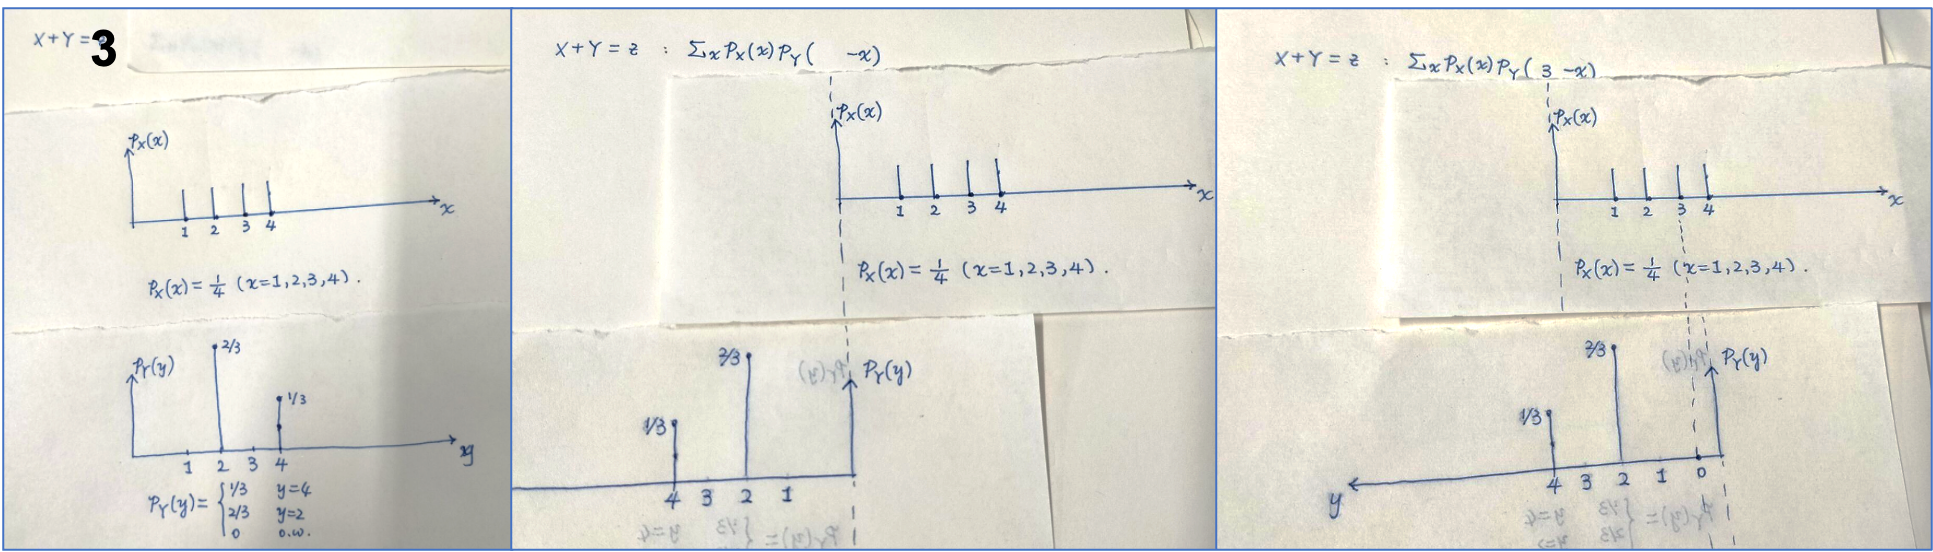
\includegraphics[width=\textwidth]{fig/ch3/convolution.png}
    \caption{直观理解卷积}
    \label{fig:convolution}
\end{figure}

\paragraph{(二)$Z=Y/X,Z=XY$的分布}

设 $(X, Y)$ 是二维连续型随机变量, 它具有概率密度 $f_{X,Y}(x, y)$.连续型随机变量$Z=Y/X$的概率密度是多少?

我们还是还是首先设出$F_{Y/X}(z)=P\{Y/X\leq z\}$. 但是这里由于函数的不连续性, 需要分两种情况: $x<0, x>0$分别考虑:

$$
\begin{aligned}
F_{Y / X}(z) & =P\{Y / X \leq z\}=\iint_{\stackrel{y / x \leq z}{x<0}} f(x, y) \mathrm{d} y \mathrm{~d} x+\iint_{\stackrel{y / x \leq z}{x>0}} f(x, y) \mathrm{d} y \mathrm{~d} x \\
& =\int_{-\infty}^0\left[\int_{z x}^{\infty} f(x, y) \mathrm{d} y\right] \mathrm{d} x+\int_0^{\infty}\left[\int_{-\infty}^{z x} f(x, y) \mathrm{d} y\right] \mathrm{d} x \\
& \varsub{y:=xu}{1cm} \int_{-\infty}^0\left[\int_z^{-\infty} x f(x, x u) \mathrm{d} u\right] \mathrm{d} x+\int_0^{\infty}\left[\int_{-\infty}^z x f(x, x u) \mathrm{d} u\right] \mathrm{d} x \\
& =\int_{-\infty}^0\left[\int_{-\infty}^z(-x) f(x, x u) \mathrm{d} u\right] \mathrm{d} x+\int_0^{\infty}\left[\int_{-\infty}^z x f(x, x u) \mathrm{d} u\right] \mathrm{d} x \\
& =\int_{-\infty}^z\left[\int_{-\infty}^+\infty|x| f(x, x u) \mathrm{d} u\right] \mathrm{d} x
\end{aligned}
$$

遵循同样的模式, 同样可以求出: $Z=XY$的概率分布. 
$$
\begin{aligned} & F_{XY}(z)=P\{XY\leq z\}\\
 & =\iint_{\substack{xy\leq z\\
 x<0}}f(x,y)\dd y\dd x+\iint_{\substack{xy\leq z\\
 x>0}}f(x,y)\dd y\dd x\\
 & =\int_{-\infty}^{0}\left(\int_{z/x}^{+\infty}f(x,y)\dd y\right)\dd x+\int_{0}^{+\infty}\left(\int_{-\infty}^{z/x}f(x,y)\dd y\right)\dd x\\
 & \varsub{y:=u/x}{1.5cm}\int_{-\infty}^{0}\left(\int_{z/x}^{+\infty}f\left(x,\frac{u}{x}\right)d\left(\frac{u}{x}\right)\right)\dd x+\int_{0}^{+\infty}\left(\int_{-\infty}^{z/x}f\left(x,\left(\frac{u}{x}\right)\dd x\right)\right)\\
 & =\int_{-\infty}^{0}\left(\left(\frac{1}{x}\right)\int_{z}^{-\infty}f\left(x,\frac{u}{x}\right)\dd u\right)\dd x+\int_{0}^{+\infty}\left(\frac{1}{x}\int_{-\infty}^{z}f\left(x,\frac{u}{x}\right)\dd u\right)\dd x\\
 & =\int_{0}^{z}\left(\int_{-\infty}^{\infty}\frac{1}{|x|}f\left(x,\frac{u}{x}\right)\dd u\right)\dd x
\end{aligned}
$$

\paragraph{(三) $M=\min \{X, Y\}$的分布}

$X, Y$ 是两个\emph{相互独立}的随机变量, 它们的分布函数分别为 $F_X(x)$ 和$F_Y(y)$.求 $M=\min \{X, Y\}$的分布函数.


   $$
\begin{aligned}
F_{\min }(z) & =P\{N \leq z\}=1-P\{N>z\} \\
& =1-P\{X>z, Y>z\}=1-P\{X>z\} \cdot P\{Y>z\}
\end{aligned}
$$

也就是
$$
F_{\min }(z)=1-\left[1-F_X(z)\right]\left[1-F_Y(z)\right] .
$$

上述的三个情况都可以推广到$n$维的情形.



\end{document}


